\documentclass[journal]{IEEEtran}
\usepackage[justification=centering]{caption}
\usepackage{float}
\usepackage{blindtext}
\usepackage{graphicx}
\usepackage[utf8]{inputenc}
\usepackage{placeins}
\usepackage[font={small}]{caption}
\setlength{\textfloatsep}{0.2cm}
\setlength{\floatsep}{0.2cm}
\setlength{\intextsep}{0.2cm}
% \setlength\floatsep{1.25\baselineskip plus 3pt minus 2pt}
% \setlength\textfloatsep{1.25\baselineskip plus 3pt minus 2pt}
% \setlength\intextsep{1.25\baselineskip plus 3pt minus 2 pt}


% Check [*

\title{Exploring the Effectiveness of Consumer Grade EEGs and EMGs as Control Inputs for Robotic Systems}
\author{A. Bennett \\ A. Elsen, B. Liebson}
%\author{A. Bennett,~%
%        A. Elsen,~%
%        and~% 
%        B. Liebson% <-this % stops a space
%        }
\date{April 2015}

\begin{document}

\maketitle

\begin{abstract}
Electroencephalograms and electromyographs are devices used most commonly in exploratory research, and medical fields such as diagnostics and rehabilitation. This study investigates the accuracy of consumer-grade EEG and EMG devices, specifically the accuracy of the Neurosky Mindwave and the Thalmic Myo. Volunteers were recruited and asked to perform specific tests and gestures for each device. During these tests, the accuracy of the devices' built-in algorithms were recorded, along with the raw EEG and EMG data. These raw samples were processed using custom MATLAB scripts, to determine the correlation of signals between volunteers for each test. The built-in algorithms of the EEG device used in this study was found to be lacking in effectiveness for any use that requires a high degree of accuracy, or a variety of inputs. The built-in gesture recognition algorithms of the EMG device proved to be fairly accurate, with a mean accuracy well above 50\% for each gesture. Results of the experiment found that the algorithm's accuracy increased up to a mean of 90\% for users with smaller wrist circumferences. The raw data from the EMG device was correlated between volunteers, and mean signals were generated from the shifted samples. These mean signals exhibited noticeable differences in shape, length, and amplitude for each gesture.
\end{abstract}

\raggedbottom
\section{Introduction}
A variety of brain-machine interfaces (BMIs) have been developed in recent years that allow animals or humans, after intensive training, to control computer displays or robots.  While several approaches have been used, non-invasive control is  less common. Our work employs only non-invasive techniques in order to reduce risk of danger for our human subjects.
The goal of this project is to investigate the

This research experiment investigates the accuracy of commercial-grade EEG and EMG devices. In this study, we compare both EEG and EMG measurements taken from volunteers, quantifying the differences of the signals as the volunteers perform specific gestures, by determining statistical correlations between an input action we ask of the subject and respective signals. By quantifying their differences and similarities, we hope to gain some insight into the factors that determine the accuracy of the device’s gesture-determination algorithms, and how these algorithms can be further improved. 

\section{Methods}
\subsection{Equipment}
\subsubsection{Electroencephalographic Device Setup}
Twenty subjects participate in the first experiment involving the EEG device.
The apparatus consists of:
\begin{itemize}
    \item \textit{Electoencephalographic (EEG) recording equipment}: The EEG recording system is a Neurosky Mindwave Mobile. The Mindwave is a consumer-grade EEG that measures signals through a singular electrode on the front of the forehead. The headset comes programmed with the manufacturer’s NeuroSky eSense, amplification off head detection, and noise filtering for EMG and 50/60HZ AC powerline interference. 
    \item \textit{Data acquisition program}: A custom MATLAB data acquisition programs using NeuroSky drivers store data in a format compatible with BCI2000 and with MATLAB.  The data acquisition program measures and records EEG data in order to compare signals across subjects.
\end{itemize}

\subsubsection{Electromyographic Device Setup}
Twenty subjects participated in the second experiment involving the EMG device.
The apparatus consists of: 
\begin{itemize}
    \item \textit{Electromyographic (EMG) recording equipment}: The EMG recording device is a Thalmic Myo. The Myo is a noninvasive armband that measures EMG signals through eight electrodes around the thickest part of the forearm. It also measures acceleration and orientation with an accelerometer and gyroscope. Using the manufacturer's software, the device also has the ability to detect six pre-programmed gestures.
    \item \textit{Data acquisition program}: A custom python data acquisition script was created using pre-existing open-source scripts. The data acquisition scripts communicate with the Myo to retrieve the raw EMG data. Data analysis scripts were also created to normalize and compare the EMG signals of each electrode, both across subjects and across data measurement sessions. Signals were compared using MATLAB's built in cross-correlation functions.
\end{itemize}
   
\subsection{Human Subjects}
\subsubsection{Characteristics and Recruitment}
The proposed study included a gender-balanced group of 20 healthy adults, ages 18-60, who were right-handed and are without any sensory, motor, or developmental deficits. Subjects were recruited from among Olin students and staff using advertisements and word of mouth. Each subject were asked to commit up to 1 hour of participation and will not be compensated. Subjects were allowed to drop out of the study without penalty.
The proposed ad is as follows: \par

\vspace{5mm}

\scriptsize 
\textit{ANTONIA AND BRIAN ARE SEEKING VOLUNTEERS WHO ARE 18-60 YEARS OF AGE, RIGHT-HANDED, AND IN GOOD HEALTH FOR A STUDY OF THE RELATIONSHIP BETWEEN WRIST MOVEMENTS/CONCENTRATION WITH THE ACCOMPANYING EEG/EMG, RESPECTIVELY. EEG AND EMG ARE NON-INVASIVE RECORDING OF ELECTRICAL ACTIVITY OF THE BRAIN AND FOREARM, RESPECTIVELY, BOTH DONE WITH SURFACE ELECTRODES. EACH SUBJECT WILL PARTICIPATE IN ONE EXPERIMENTAL SESSION LASTING UP TO 1 HOUR AND WILL NOT BE COMPENSATED. IF INTERESTED, E-MAIL brian@students.olin.edu or antonia.elsen@students.olin.edu FOR AN APPOINTMENT.} 

\vspace{5mm}
\normalsize Subjects who responded to the ad were asked to confirm that they fit the age and health requirements of the study, and were invited to make an appointment. See Appendix A. No special or vulnerable populations were used.

\subsubsection{Risk and Consent}
Regarding the designation of risk in this Protocol, we go by the Code of Federal Regulations (Title 45, § 46.102), according to which if the level of discomfort or the possibility of harm is no higher than in everyday life, the experiment is a \textbf{minimal risk}. The one specific item one does not routinely encounter in everyday life is the EEG recording procedure with a headset which involves a minor inconvenience due to the pressure it may cause around the ears. \par
Subjects were recruited by advertisements and screened by phone. Subjects who meet the inclusion/exclusion criteria (Appendix A) were offered to schedule an appointment. When the subject came to the lab at the appointed time, he/she was accompanied into the experimental room where the testing was conducted. The experimental setup and the relevant equipment was be shown and explained. During this time, the experimenter ascertained whether the subject reads English well enough to understand the informed consent documents. Subjects for whom English is not the primary language were not used. The subject was then given the Experiment Description and Consent Form to read (see Appendices B). Subjects was encouraged to ask any questions they may have had.  Next, they were asked to read and sign the Consent Form. \par  A copy of the signed consent form was given to the subject; the original was scanned and kept in cloud storage, shared only between the researchers and strict confidence was kept with regard to all subjects’ information and collected data.
For information about the study, subjects were encouraged to contact study directors, and with questions about their rights as research participants, to contact Brandeis Committee for Protection of Human Subjects with specific contact information.   

\subsection{Signal Acquisition}
\subsubsection{Signal Acquisition - EEG}
Twenty subjects participate. Each subject will don the Mindwave Movile, and be asked to perform a number of tests. The first is the subject to concentrate at an object in the room for 20 seconds. The second is the subject to meditate for 20 seconds. The raw EEG bands (Delta, Theta, Alpha, Beta, Gamma, and Mu) as well as NeuroSky’s self-defined concentration and meditation levels will be recorded in MATLAB.: numerical outputs on 0-100 scales. Third, the subject will sit until the subject blinks 20 times. The researchers will visually record blinking and compare to the MATLAB recorded number. After a short break, this cycle will repeat three times in the order of concentration, blinking, meditation, and a break in order to give the subject a larger break between concentration and meditation. The research assistants will be verbally leading the subject through these tests. This entire experiment per subject will take approximately ten minutes.

\subsubsection{Signal Acquisition - EMG}
Seventeen subjects participate. Each subject will don the Myo and perform the built-in Thalmic calibration routine. This calibration routine trains the subject to perform four built-in gestures. The subject will be asked to perform each of the four gestures ten times, to determine the accuracy of Thalmic's gesture recognition algorithms. Then, the volunteer is asked to perform these same four gestures again, eight times each, as a python script records the raw EMG data taken from the Myo. This data acquisition procedure takes approximately ten minutes.

\section{Results}
\subsection{EEG Results} \par
\subsubsection{Big Picture Results}
These are the results about Neurosky's eSense Meter for "Attentiveness" and "Meditation" readings that are created with a non-public algorithm. In addition, these results begin to discuss the accuracy in measuring subject blinks.

\begin{figure}[H]
    \centering
    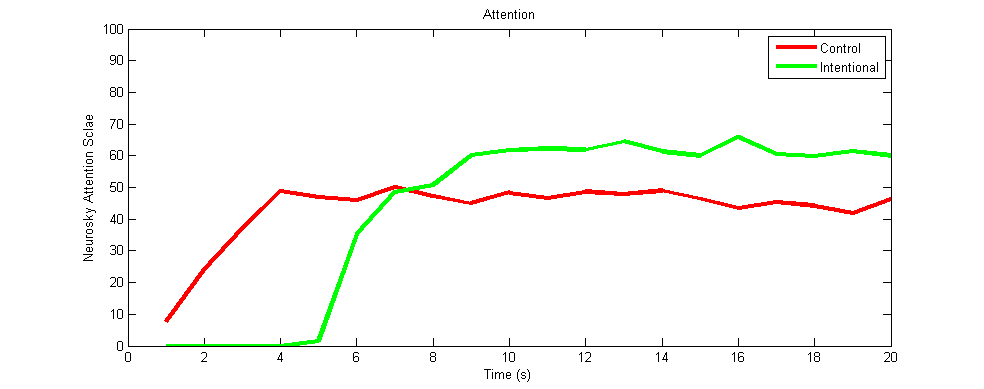
\includegraphics[width=.5\textwidth]{EEG/Attention}
    \caption{eSense Attention Readings}
    \label{attention}
\end{figure}

\begin{figure}[H]
    \centering
    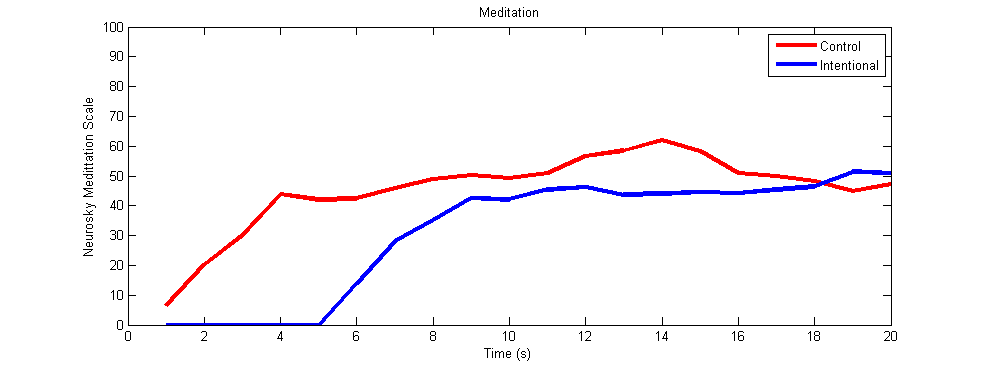
\includegraphics[width=.5\textwidth]{EEG/Meditation}
    \caption{eSense Meditation Readings}
    \label{meditation}
\end{figure} 

In order to analyze the signals, all of the subject's attention readings were averaged out at each time step. The intentional attention readings came from the "focusing on an object" test and the control readings came from the "blinking" test. Similarly goes with the meditation with the "relaxing" test in place of the "focusing on an object" test. \par 

Fig. \ref{attention} appears to show that the attention readings are clearly elevated when people are intentionally attentive. The mean for intentional attention is 61.751 with a standard deviation of 1.9266 when sampling from seconds 10-20 while the mean for unintentional, or control, attention is 46.1773 with a standard deviation of 2.2798 based on the same time scale. This time period was used in order to avoid the skewed beginning data sliding up from 0. Note: these units are somewhat unknown, based on a 0-100 scale created by an algorithm from the Neurosky Company. By these standards, we'd expect the conclusion to be that this EEG is fairly effective in being able to detect attentiveness, specifically intentionally. \par

In Fig. \ref{meditation}, the meditation readings are less directly contrasting, they even cross over at the end. Nonetheless, the mean for intention meditation is 45.8545 with a standard deviation of 2.8718 and the mean for control meditation is 52.4364 with a standard deviation of 5.4695, both sampled from 10-20 seconds. Perhaps the intentional meditation was lower on the meditation scale because "concentrating" on meditation is an odd task. That being said, the means are definitely different, and while not as contrasting as the attention means, the standard deviation seems to make this difference seem somewhat significant. It is very curious that the lines cross over at the end, however. It seems as if this data might be flawed in a way that these graphs are not the best representation to show what the results say.  \par

\begin{figure}[H]
    \centering
    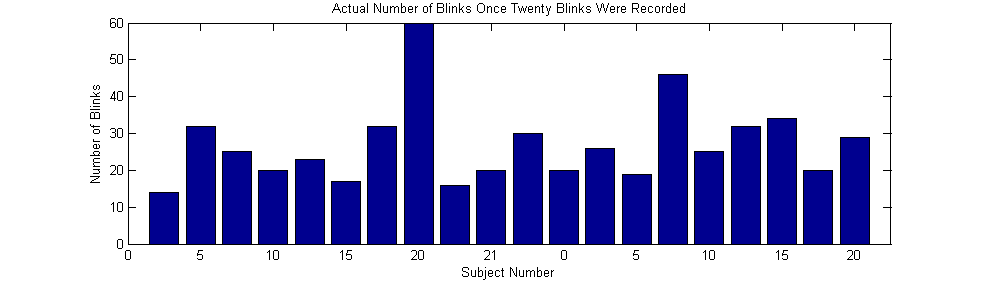
\includegraphics[width=.5\textwidth]{EEG/Actual_blinks_graph}
    \caption{Blinking Data}
    \label{blinking}
\end{figure} 

Fig. \ref{blinking} shows how many times a subject was asked to blink before the program outputted that he or she had blinked 20 times. The average number of blinks being incorrect in either direction was 8.4 across 20 people. The normal mean is 7, indicating that the subject blinked 7 more blinks on average that were not recorded. The average offset from 20 was 35 percent. \par

The raw data from every subject was then plotted in the graphs below to attempt to visualize some sorts of correlation: \par

\begin{figure}[H]
    \centering
    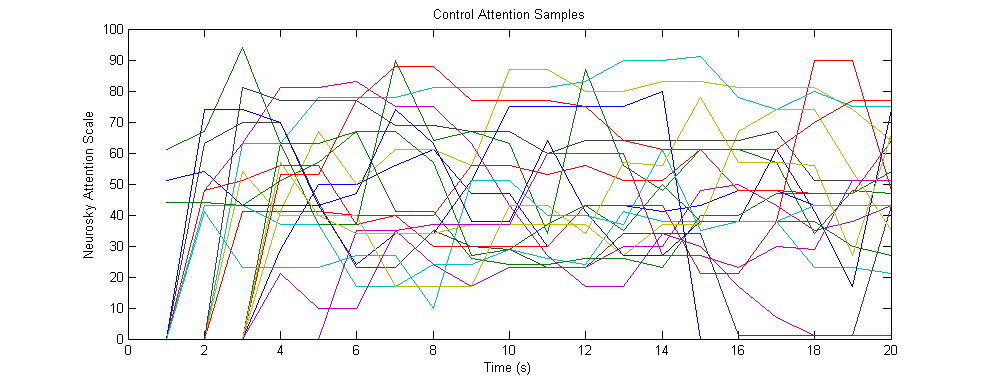
\includegraphics[width=.5\textwidth]{EEG/all_attentions_control}
    \caption{Raw Control Attention Readings}
    \label{a_a_c}
\end{figure} 

\begin{figure}[H]
    \centering
    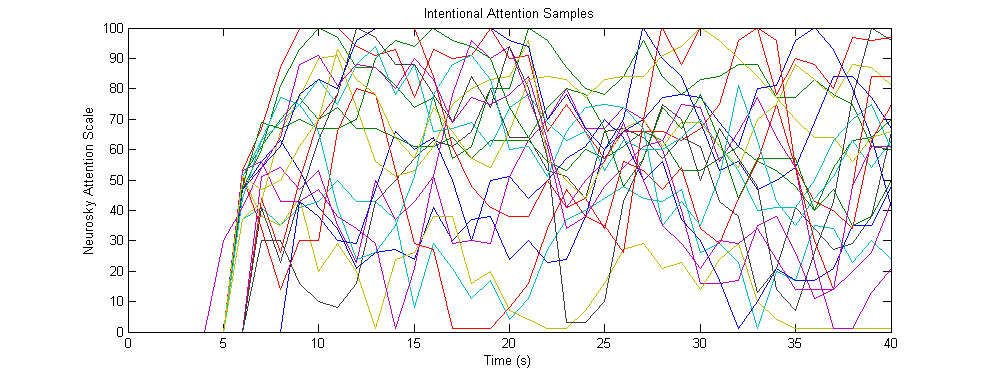
\includegraphics[width=.5\textwidth]{EEG/all_attentions_intentional}
    \caption{Raw Intetntional Attention Readings}
    \label{a_a_i}
\end{figure} 


Sadly, these graphs are simply madness and spiderwebs. Each color represents one of twenty test subjects. While averaging out the data earlier gave clean, simple, and seemingly useful and significant numbers, fig. \ref{a_a_c} shows that there was not really any sort of correlation or kind of baseline as a control. The same goes with fig. \ref{a_a_i}. The only notable difference between the graphs is that in fig. \ref{a_a_i}, the amplitude is more extreme reaching the maximum and minimum, while fig. \ref{a_a_c}'s assortment of waves stays smaller and closer to the middle. There is no obvious correlation here. \par

\begin{figure}[H]
    \centering
    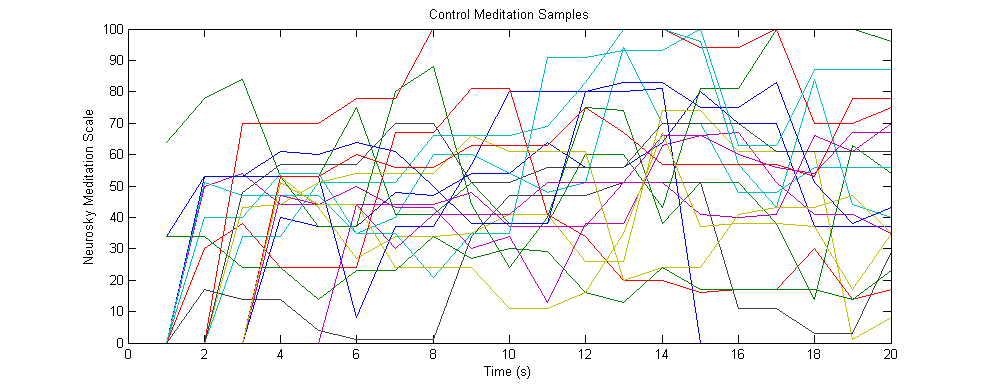
\includegraphics[width=.5\textwidth]{EEG/all_meditations_control}
    \caption{Raw Control Meditation Readings}
    \label{a_m_c}
\end{figure} 

\begin{figure}[H]
    \centering
    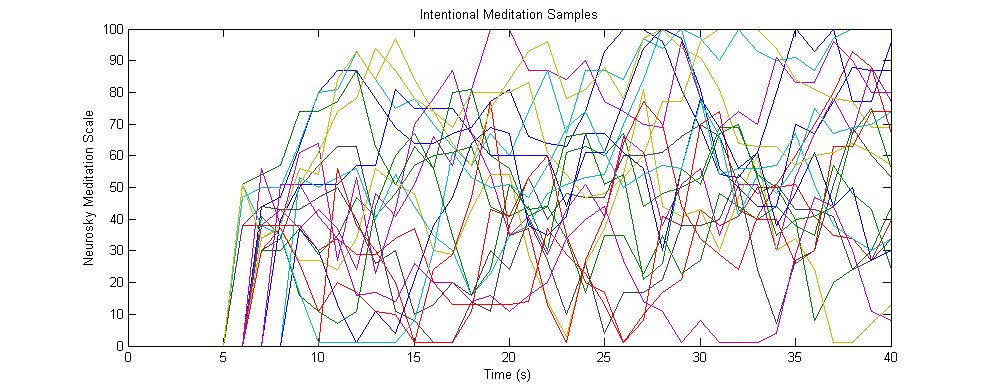
\includegraphics[width=.5\textwidth]{EEG/all_meditations_intentional}
    \caption{Raw Intetntional Meditation Readings}
    \label{a_m_i}
\end{figure}


Similarly goes with the pair of meditation graphs. Once again, fig. \ref{a_m_c} and fig. \ref{a_m_i} show "spaghetti graphs" with numbers anywhere. The only significant difference is the control seems to be more stable, but only looks that way due to the different time axes. Both graphs show the ineffectiveness is recording meditation data. \par

\vspace{5mm}

\subsubsection{Wave Results}
These are the results that analyze the individual brain waves (Delta, Gamma, Theta, etc.) that Neurosky measures but does not use an algorithm to alter. In the following graphs, there is no y axis, common amongst these types of representations. Assume the y axis is how present or strong the signal is. \par

\begin{figure}[H]
    \centering
    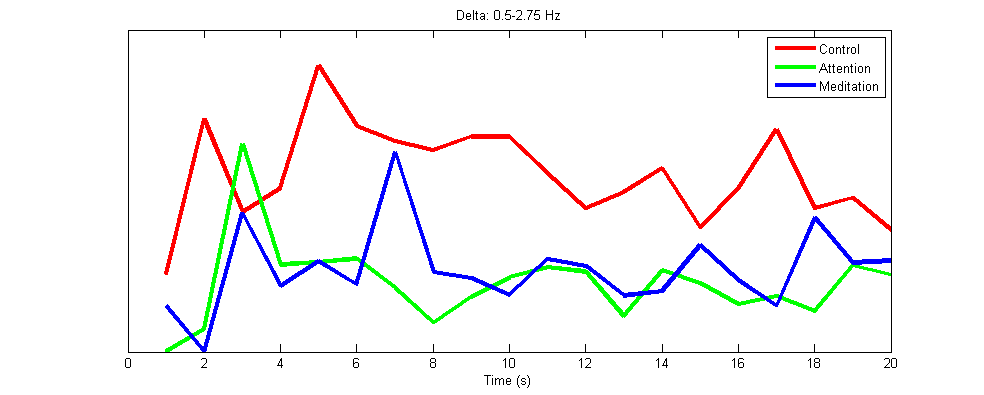
\includegraphics[width=.5\textwidth]{EEG/wave1}
    \caption{Delta Wave Averages}
    \label{w1}
\end{figure}

\begin{figure}[H]
    \centering
    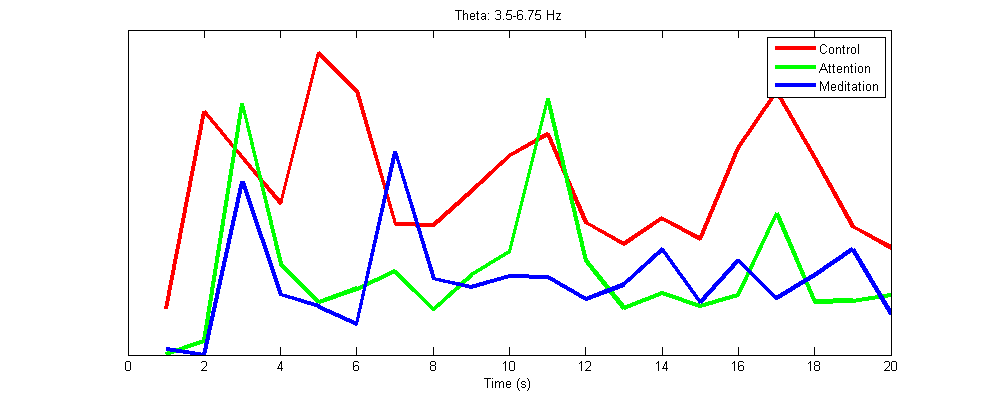
\includegraphics[width=.5\textwidth]{EEG/wave2}
    \caption{Theta Wave Averages}
    \label{w2}
\end{figure}

\begin{figure}[H]
    \centering
    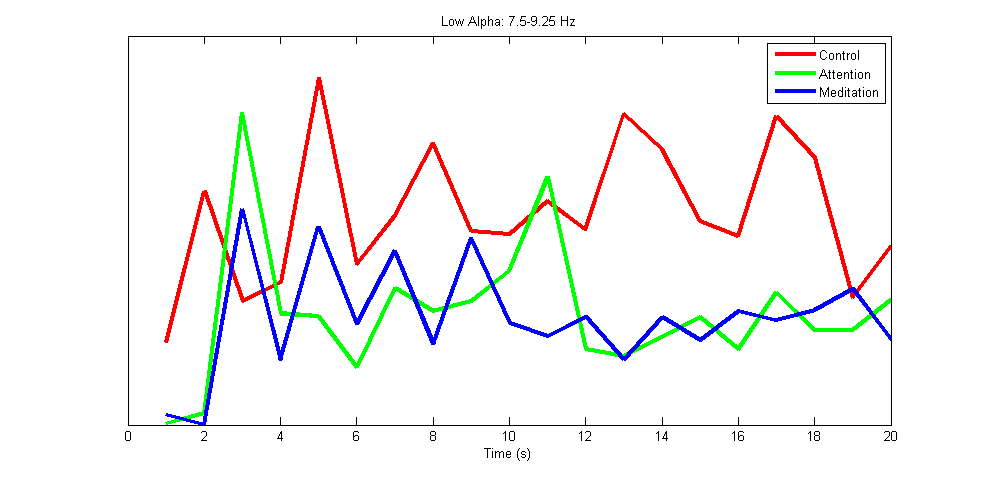
\includegraphics[width=.5\textwidth]{EEG/wave3}
    \caption{Low Alpha Wave Averages}
    \label{w3}
\end{figure}

\begin{figure}[H]
    \centering
    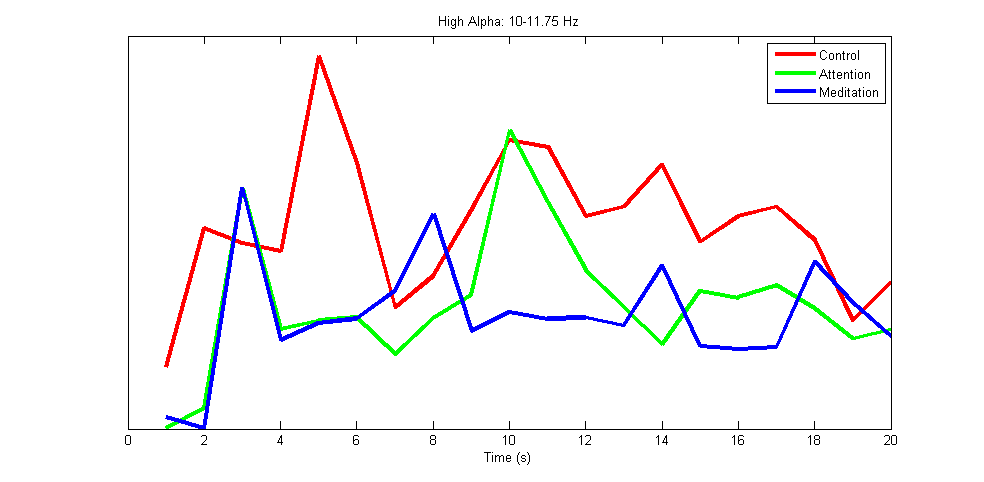
\includegraphics[width=.5\textwidth]{EEG/wave4}
    \caption{High Alpha Wave Averages}
    \label{w4}
\end{figure}

\begin{figure}[H]
    \centering
    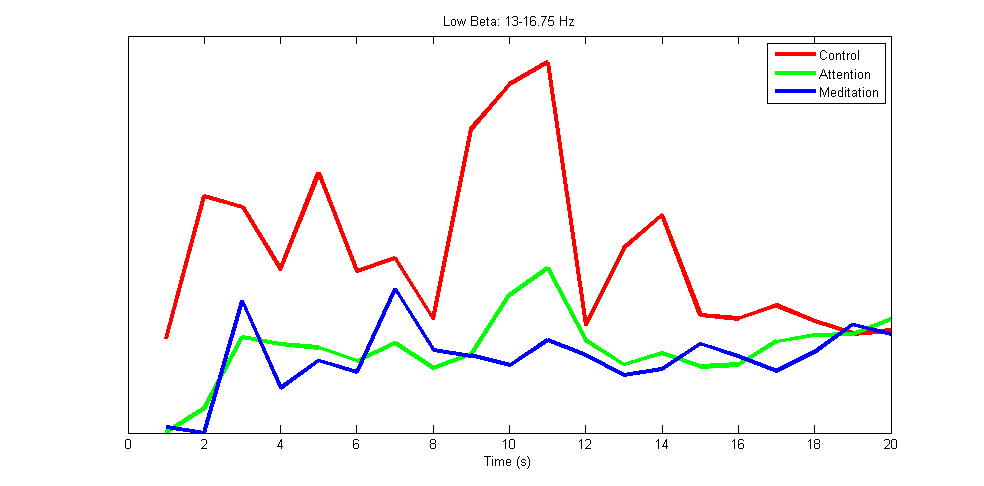
\includegraphics[width=.5\textwidth]{EEG/wave5}
    \caption{Low Beta Wave Averages}
    \label{w5}
\end{figure}

\begin{figure}[H]
    \centering
    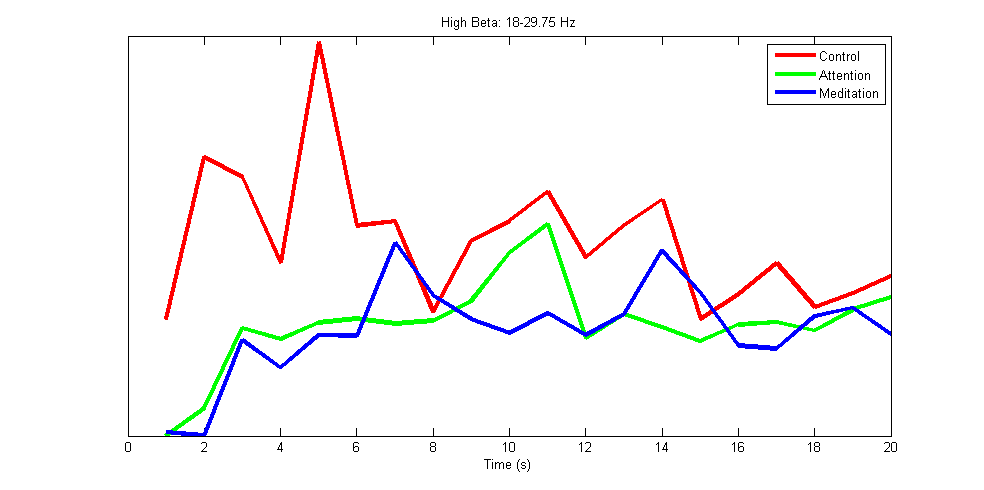
\includegraphics[width=.5\textwidth]{EEG/wave6}
    \caption{High Beta Wave Averages}
    \label{w6}
\end{figure}

\begin{figure}[H]
    \centering
    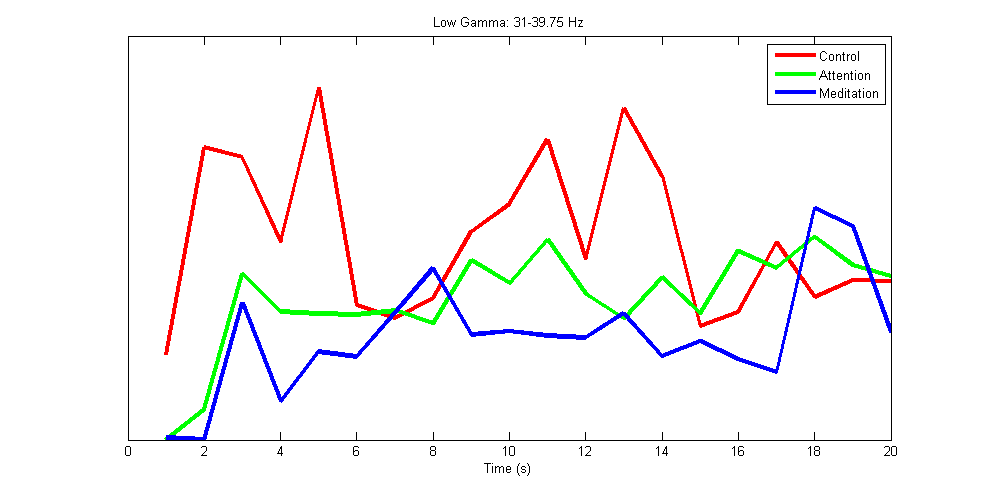
\includegraphics[width=.5\textwidth]{EEG/wave7}
    \caption{Low Gamma Wave Averages}
    \label{w7}
\end{figure}

\begin{figure}[H]
    \centering
    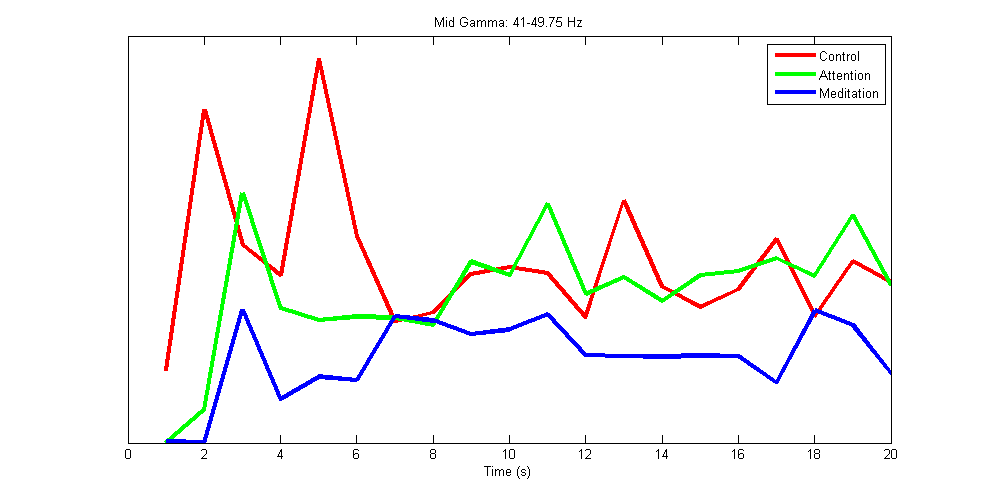
\includegraphics[width=.5\textwidth]{EEG/wave8}
    \caption{Mid Gamma Wave Averages}
    \label{w8}
\end{figure}


Amongst all these graphs, it appears that the control signal, in red, is always the upper bounds of the lines. There is a plethora of data suggesting certain signals being related to certain actions. For example, fig. \ref{w1}'s Delta signal is suggested to pertain to unconscious and resting behaviors. It is expected that there should be visual excitement regarding the meditation or attention lines: very obvious separations of lines. That being said, a similar conclusion was met in the big picture results section previously. \par

\begin{figure}[H]
    \centering
    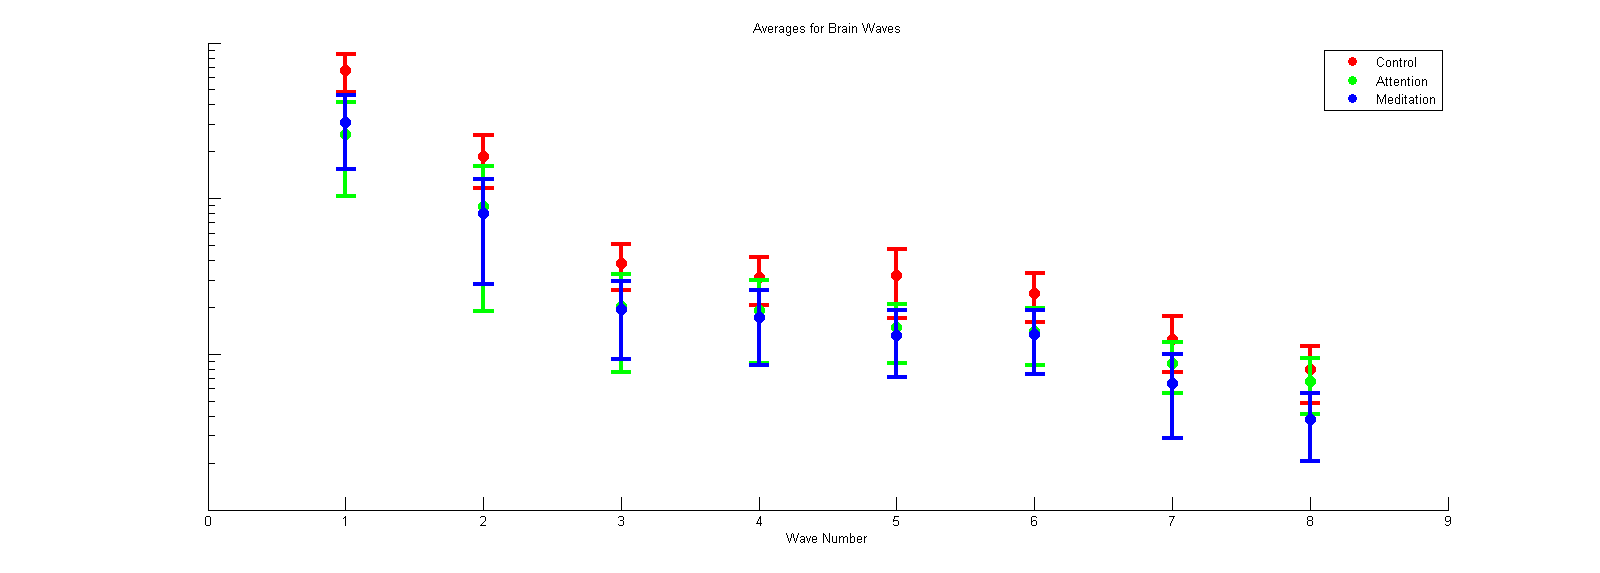
\includegraphics[width=.5\textwidth]{EEG/wave_averages}
    \caption{Wave Means with Standard Deviations}
    \label{w_av}
\end{figure} 

The data may be more easily visualized here. The means of each wave for control, attention, and meditation were recorded and standard deviations were calculated for the bars. Evidently, the numbers are not significantly different in any wave regardless of the task. The means and standard deviations can be found below for curiosity sake. The units are unknown, but definitely a notation of how strong the signal is. Note: Waves are ordered 1-8 beginning with Delta and ending with Mid Gamma.

    \begin{center}
    \begin{tabular}{||c c c c c c c||} 
    \hline
    Wave & Con Mean & Att Mean & Med Mean \\ [0.5ex] 
    \hline\hline
    1 & 6.83E5 & 2.53E5 & 3.22E5 \\ 
    \hline
    2 & 1.87E5 & 8.86E4 & 8.27E4 \\
    \hline
    3 & 4.04E4 & 2.03E4 & 2.03E4 \\
    \hline
    4 & 3.27E4 & 2.02E4 & 1.79E4 \\
    \hline
    5 & 3.19E4 & 1.62E4 & 1.41E4 \\
    \hline
    6 & 7.85E3 & 7.17E3 & 4.14E3 \\
    \hline
    7 & 1.23E4 & 9.56E3 & 7.08E3 \\
    \hline
    8 & 7.85E3 & 7.17E3 & 4.14E3 \\ [1ex] 
    \hline
    \end{tabular}

    \end{center}
    


\begin{center}
 \begin{tabular}{||c c c c c c c||} 
 \hline
 Wave & Con Std. & Att Std. & Med Std. \\ [0.5ex] 
 \hline\hline
 1 & 1.61E5 & 7.56E4 & 1.35E5 \\ 
 \hline
 2 & 6.50E4 & 5.54E4 & 4.17E4 \\
 \hline
 3 & 1.14E4 & 7.83E4 & 7.15E4 \\
 \hline
 4 & 1.02E4 & 8.43E3 & 5.51E3 \\
  \hline
 5 & 1.57E4 & 4.68E3 & 4.05E3 \\
  \hline
 6 & 8.19E3 & 3.85E3 & 4.09E3 \\
  \hline
 7 & 4.64E4 & 1.81E3 & 3.09E3 \\
 \hline
 8 & 2.77E3 & 1.52E3 & 1.22E3 \\ [1ex] 
 \hline
\end{tabular}
\end{center}


\section{Discussion}
\subsection{EEG}
EEGs and understanding the brain is immensely complex. While the Neurosky Mindwave Mobile is not very effective at all as an EEG, it should not be expected to be very effective. Research-grade EEGs have more than simply 1 electrode on the forehead and are custom fit for each user. That being said, the company claimed their product to be an effective EEG. \par

The Neurosky algorithms, while running and producing "Attention" and "Meditation" levels, seemed to be effective to the researcher looking at the computer. This was mostly a kind of placebo-effect, where the researcher was happy when the readings were high and pushed aside the low readings, assuming the subject had lost concentration or meditation focus. However, this study was also very difficult because of the complexity of brains: intention is much different than what the brain may actually be doing. When people "try" to meditate, does this mean that the subject is being attentive because he or she is focusing on trying to meditate? This created a very difficult dilemma. In the end, the goal of this research is to explore the effectiveness of the Neurosky Mindwave Mobile, or a consumer-grade EEG, in controlling a robotic system. Because controlling attention or meditation is not simple, this system is not effective. This is not to say that the system is incorrect: it is quite possible that the Mindwave Mobile is reading the exact things it wants to, and correctly. However, the documentation about the eSense "Attention" and "Meditation" meters are discussed in simple terms with no actual suggested experiments, so what the researchers tested for "Attention" and "Meditation" levels may be completely incorrect. This is a side effect from simple lacks of documentation and a lack of support within the company. \par

For these errs, the individual waves were explored. Theoretically, when asked to be attentive or meditative, some common types of action should happen across people that should be measurable somewhere in these waves. This appeared not to be true, but should be true fundamentally: when the body does something, the brain controls it (excluding a reflex, which this is not). The lack of effectiveness is simply attributed to the Mindwave not being very effective. One of the reach goals with this project was to perhaps devise a new algorithm for the researcher's own "eSense meters" for attention and meditation. However, the lack of any fundamental results in the individual wave section means that this is not possible. \par

All in all, this was an experiment-based exploration into the effectiveness of a consumer grade EEG controlling a robotic system. The definition of success would be having results suggestion the ability to control a system: individual waves are significantly different dependent on the intention of the user. Whether this was unsuccessful due to the EEG used or the experimental design is not very relevant. The concluding remarks remind that brains are extremely complex between actual action and intention, and trying to record accurately with a cheap, non-robust system will not be effective. \par

Blinking did end up being somewhat effective, however. Most of the issues from blinking tests were from the headset not fitting properly due to its inelastic properties. Not discussed previously, blinking was very easy to get better at. Some subjects asking about the experiment and code post-testing really enjoying the blinking test, and got better with time. The data above discussed the first-time use for blinking tests; the thought in mind was if this system was going to control a robotic system, it should be very effective and accurate on the first try. That being said, getting more accurate blinks involves a very simple learning curve. Blinking is proposed to be an effective controller for robotic systems above trying to be attentive or meditative. However, this may simply be due to the fact that blinking is measured with an EEG, but is not really an EEG signal, more of an EMG signal because it measures the muscles being activated. \par

\newpage
\subsection{EMG Results}
\subsubsection{Gesture Recognition Algorithm Results} \\
Every volunteer was asked to perform each of the four gestures ten times as the built-in Thalmic gesture recognition software was run in the background. The accuracy of this recognition software was quantified by calculating the percentage of correctly recognized gestures. Finally, the mean percentage and standard deviation was calculated for each gesture. A plot of these results can be seen below, in fig. \ref{accungroup} and in table 1. The plot suggests that the mean percentage value of every gesture is approximately $80\%$ --- meaning that the software will correctly identify any given gesture four out of five times. The standard deviation is very high, suggesting that the data is relatively disjointed.

\begin{table}[h]
\resizebox{1.7\columnwidth}{!}{\begin{minipage}{\textwidth}
\begin{tabular}{ c || c | c | c | c | c }
    Arm Width	& Fist	& Spread	& Wave - Right	& Wave - Left	& Average \\
    \hline
    All & $85.29\%$ & $71.76\%$ & $84.12\%$ & $85.29\%$ & $81.62\%$ \\
    Large & $82.00\%$ & $44.00\%$ & $56.00\%$ & $72.00\%$ & $63.50\%$ \\
    Medium & $93.33\%$ & $72.22\%$ & $84.44\%$ & $84.44\%$ & $83.61\%$ \\
    Small & $92.00\%$ & $100.00\%$ & $98.00\%$ & $98.00\%$ & $97.00\%$ \\
    \end{tabular} 
\label{table:name}
\end{minipage} }
\end{table}
    
    \begin{figure}[H]
    \begin{centering}
    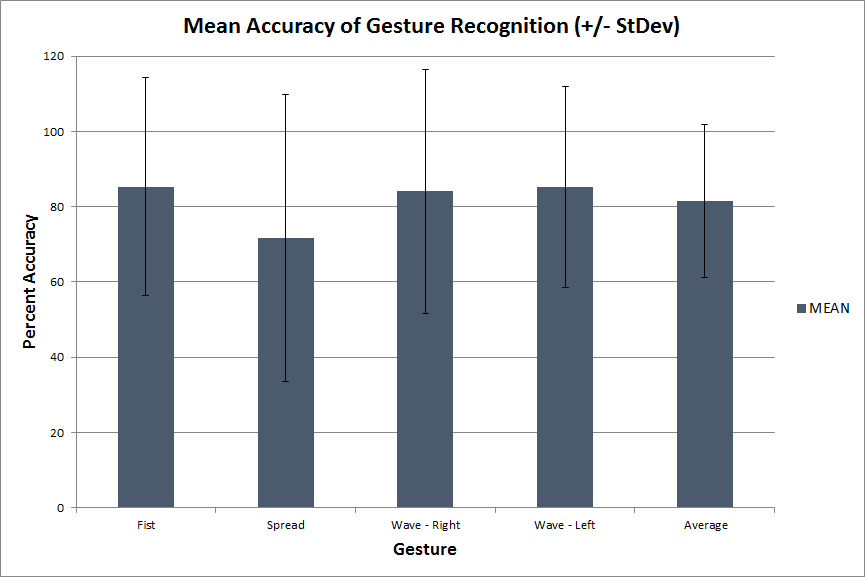
\includegraphics[width=.8\columnwidth]{EMG/Accuracy_Ungrouped}
    \caption{The accuracy (in percentage of gestures identified correct) of the built-in recognition algorithms.}
    \label{accungroup}
    \end{centering}
    \end{figure}
    
However, when we separate volunteers by forearm width, a few trends emerge. As the chart in fig. \ref{accgroup} demonstrates, the percent accuracy is noticeably higher in the volunteer group with smaller forearms, compared to the other size groups. The standard deviation of these mean values also decreases with size. This suggests that arm size may influence the ability of the algorithm to correctly guess the volunteer's performed gesture.

    \begin{figure}[H]
    \begin{centering}
    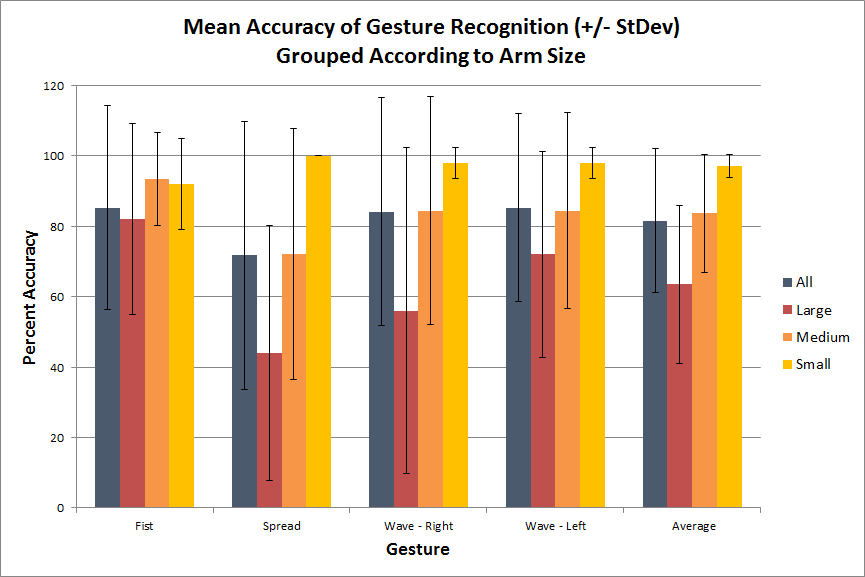
\includegraphics[width=.8\columnwidth]{EMG/Accuracy_Grouped}
    \caption{The accuracy (in percentage of gesture identified correct) of the built-in recognition algorithms, when the volunteers are sorted into groups determined by arm thickness.}
    \label{accgroup}
    \end{centering}
    \end{figure}
    
\pagebreak[4]
\newpage


\subsubsection{Raw EMG Data - Signal Correlation} \\ 
Before analyzing the raw EMG data, it was necessary to shift each EMG sample based on its correlation to a 'baseline' sample signal, or an average, due to the fact that not every gesture wavelet begins at the same time in any given sample of raw data. MATLAB's built-in function "xcorr" was used to align each sample --- first, the correlation relative to the baseline was calculated for each data point in the signal. Then, the entire sample was shifted forward or backward by the lag value of the maximum point of correlation. This was done for each sample signal of each volunteer, for each gesture. Once the batch of samples for each volunteer was shifted, a baseline signal was generated by computing the element-by-element mean each sample in the batch. \\
This correlation-shift process is illustrated in figures \ref{Spread_Min_Sahaquiel_Unshifted} - \ref{Spread_Max_Sachiel_Shifted} on pg. \pageref{Spread_Min_Sahaquiel_Unshifted}, which compare unshifted "spread" gesture samples of volunteers "Sahaquiel" (\#14) and "Sachiel" (\#13)  to their shifted results. These two volunteers were chosen because they illustrate [how correlated/uncorrelated]. Volunteer "Sahaquiel" (\#14) has the lowest mean correlation between his/her samples relative to the average of these samples for the "spread" gesture, at a mean value of 0.9176. Volunteer "Sachiel" (\#13) has the highest, at 0.9848. \\
   An example of every "spread" gesture sample from every volunteer, correlated and shifted relative to an arbitrary sample, is given in figure \ref{spread_all_correlated}. This figure demonstrates that, while the samples belonging to the same volunteer are similar in shape, amplitude, and length, they vary --- sometimes greatly --- between each volunteer. It is therefore useful to correlate samples to a computed mean (baseline) signals for each volunteer. This is done by shifting the samples for each individual volunteer to an arbitrary signal taken from the batch (ex: the first sample measured), then averaging these shifted signals to create the mean baseline, and the correlating the samples to this baseline.
    
    \begin{figure}[H]
    \centering
    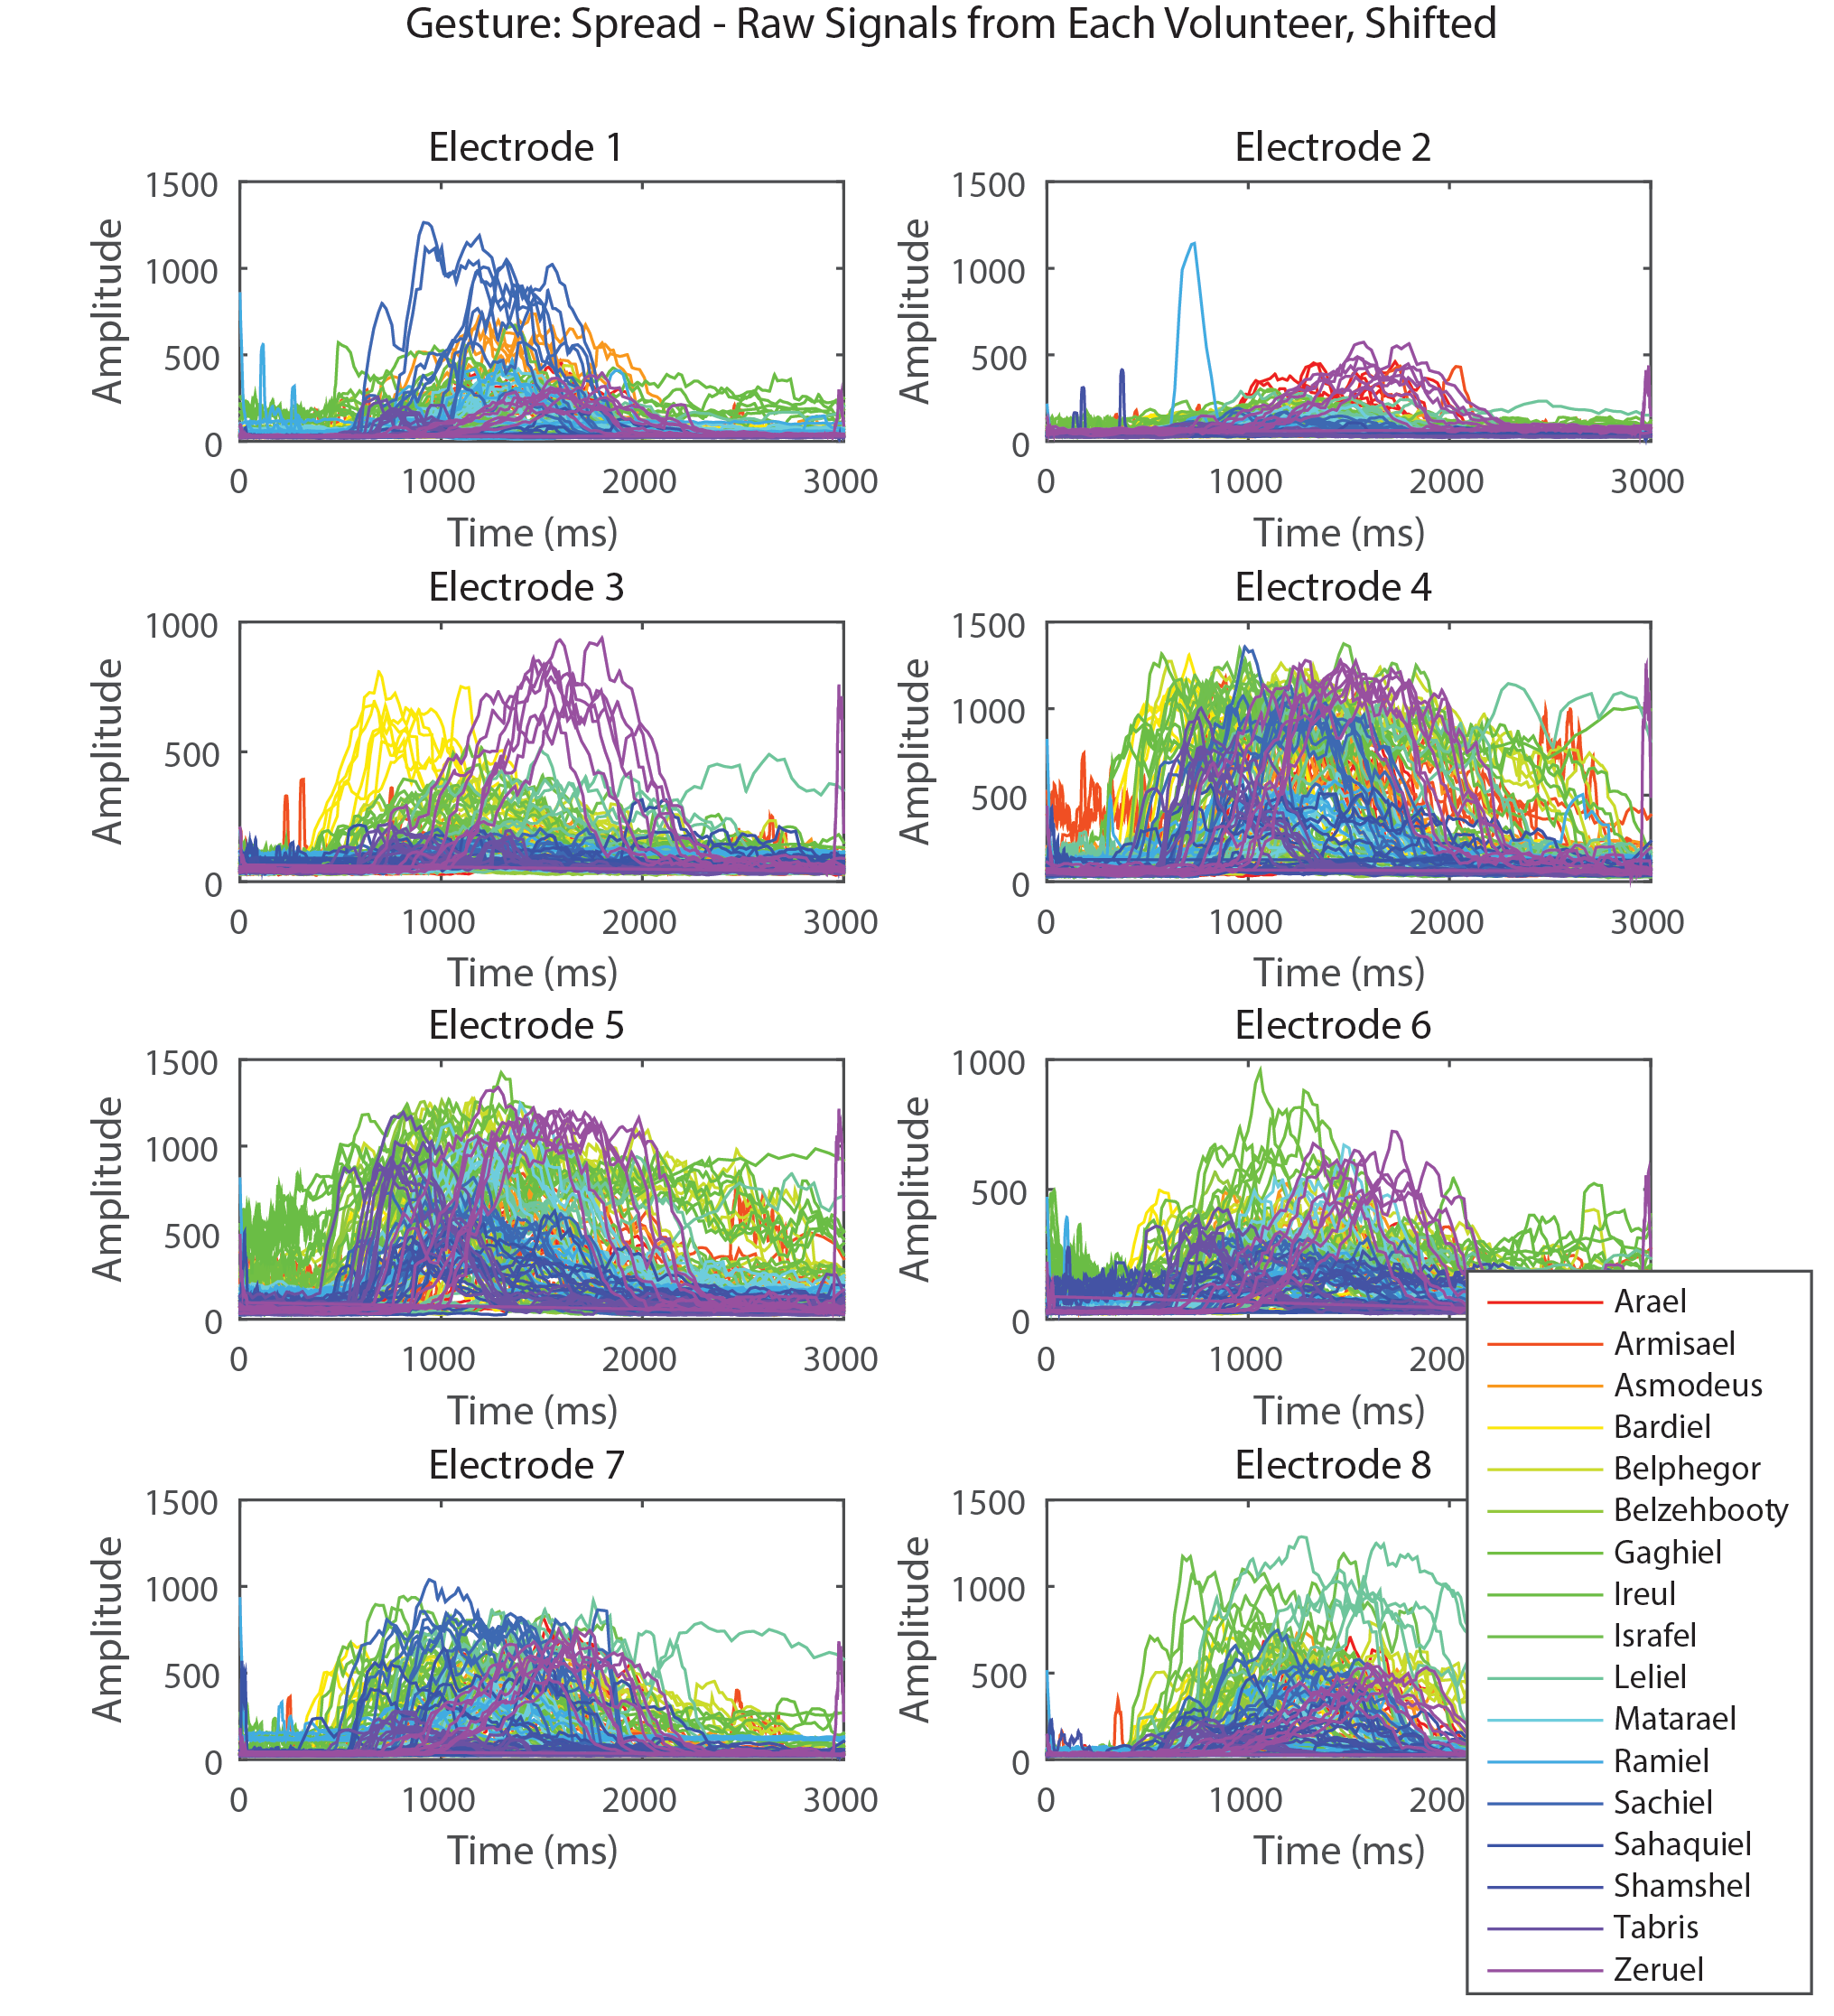
\includegraphics[width=.8\columnwidth]{EMG/spread_all_correlated}
    \caption{Samples from every volunteer for the gesture "spread", for each electrode. Each sample is shifted by determining the closest correlation to an arbitrary 'baseline'.}
    \label{spread_all_correlated}
    \end{figure}

\\
A plot of the average correlations for each volunteer and gesture, relative to their mean sample, is shown in fig. \ref{Average_Corr_Bar}. The means of these data sets is also shown in fig. \ref{Correlation_Grouped}, arranged by a qualitative assessment of volunteer arm size.

    \begin{figure}[H]
    \centering
    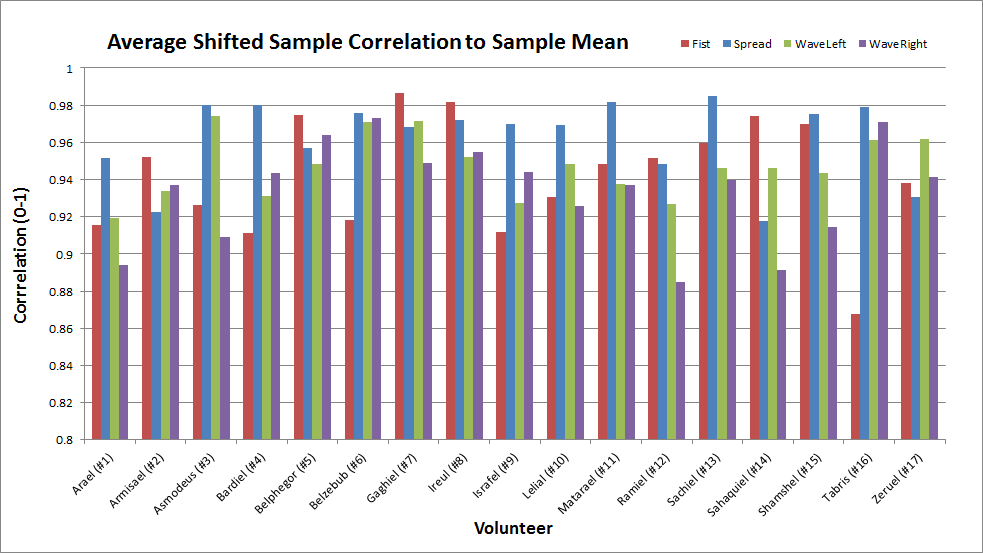
\includegraphics[width=.95\columnwidth]{EMG/Average_Corr_Bar}
    \caption{The average correlation of the samples of each volunteer for each gesture, relative to the mean of those samples.}
    \label{Average_Corr_Bar}
    \end{figure}
    
    \begin{figure}[H]
    \centering
    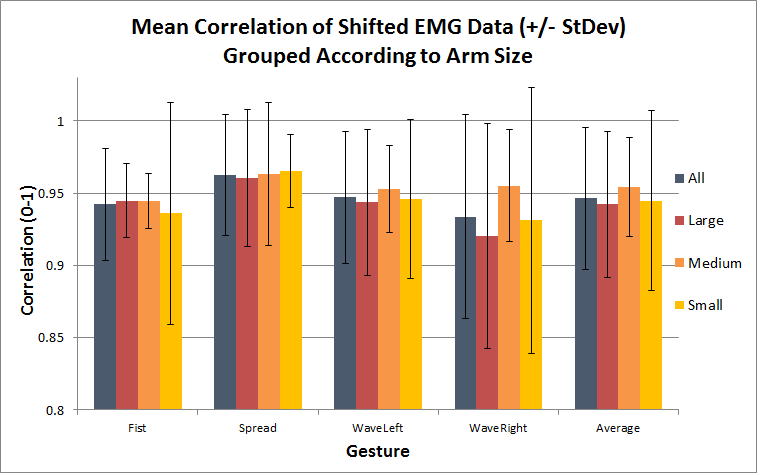
\includegraphics[width=.8\columnwidth]{EMG/Correlation_Grouped}
    \caption{The average correlation of the samples for each gesture, relative to the mean of those samples, grouped by a qualitative assessment of volunteer arm size.}
    \label{Correlation_Grouped}
    \end{figure}
    
Fig. \ref{Correlation_Grouped} suggests that the average correlation of the samples for any given volunteer does not vary greatly with arm circumference. It does show that samples taken from a volunteer with a larger arm circumference tend to correlate less with the mean of that batch, while samples from those with a smaller or medium arm circumference tend to correlate more. However, the contrast is much less distinct. 

These findings contrast with our results from the previous section, where fig. \ref{accgroup} suggested that the success rate of the Myo's gesture recognition algorithm was directly related to the circumference of the user's arm --- the smaller the circumference, the more likely the algorithm was to recognize the gesture correctly.

Finally, fig. \ref{Mean_All} demonstrates the average data from all volunteers for each gesture plotted on the same electrode graphs, to better compare and contrast the differences between the raw EMG data for each gesture.
There are qualitatively noticeable differences between the average signals of every electrode for each gesture, in both shape, amplitude, and wavelet duration. 

    \begin{figure}[H]
    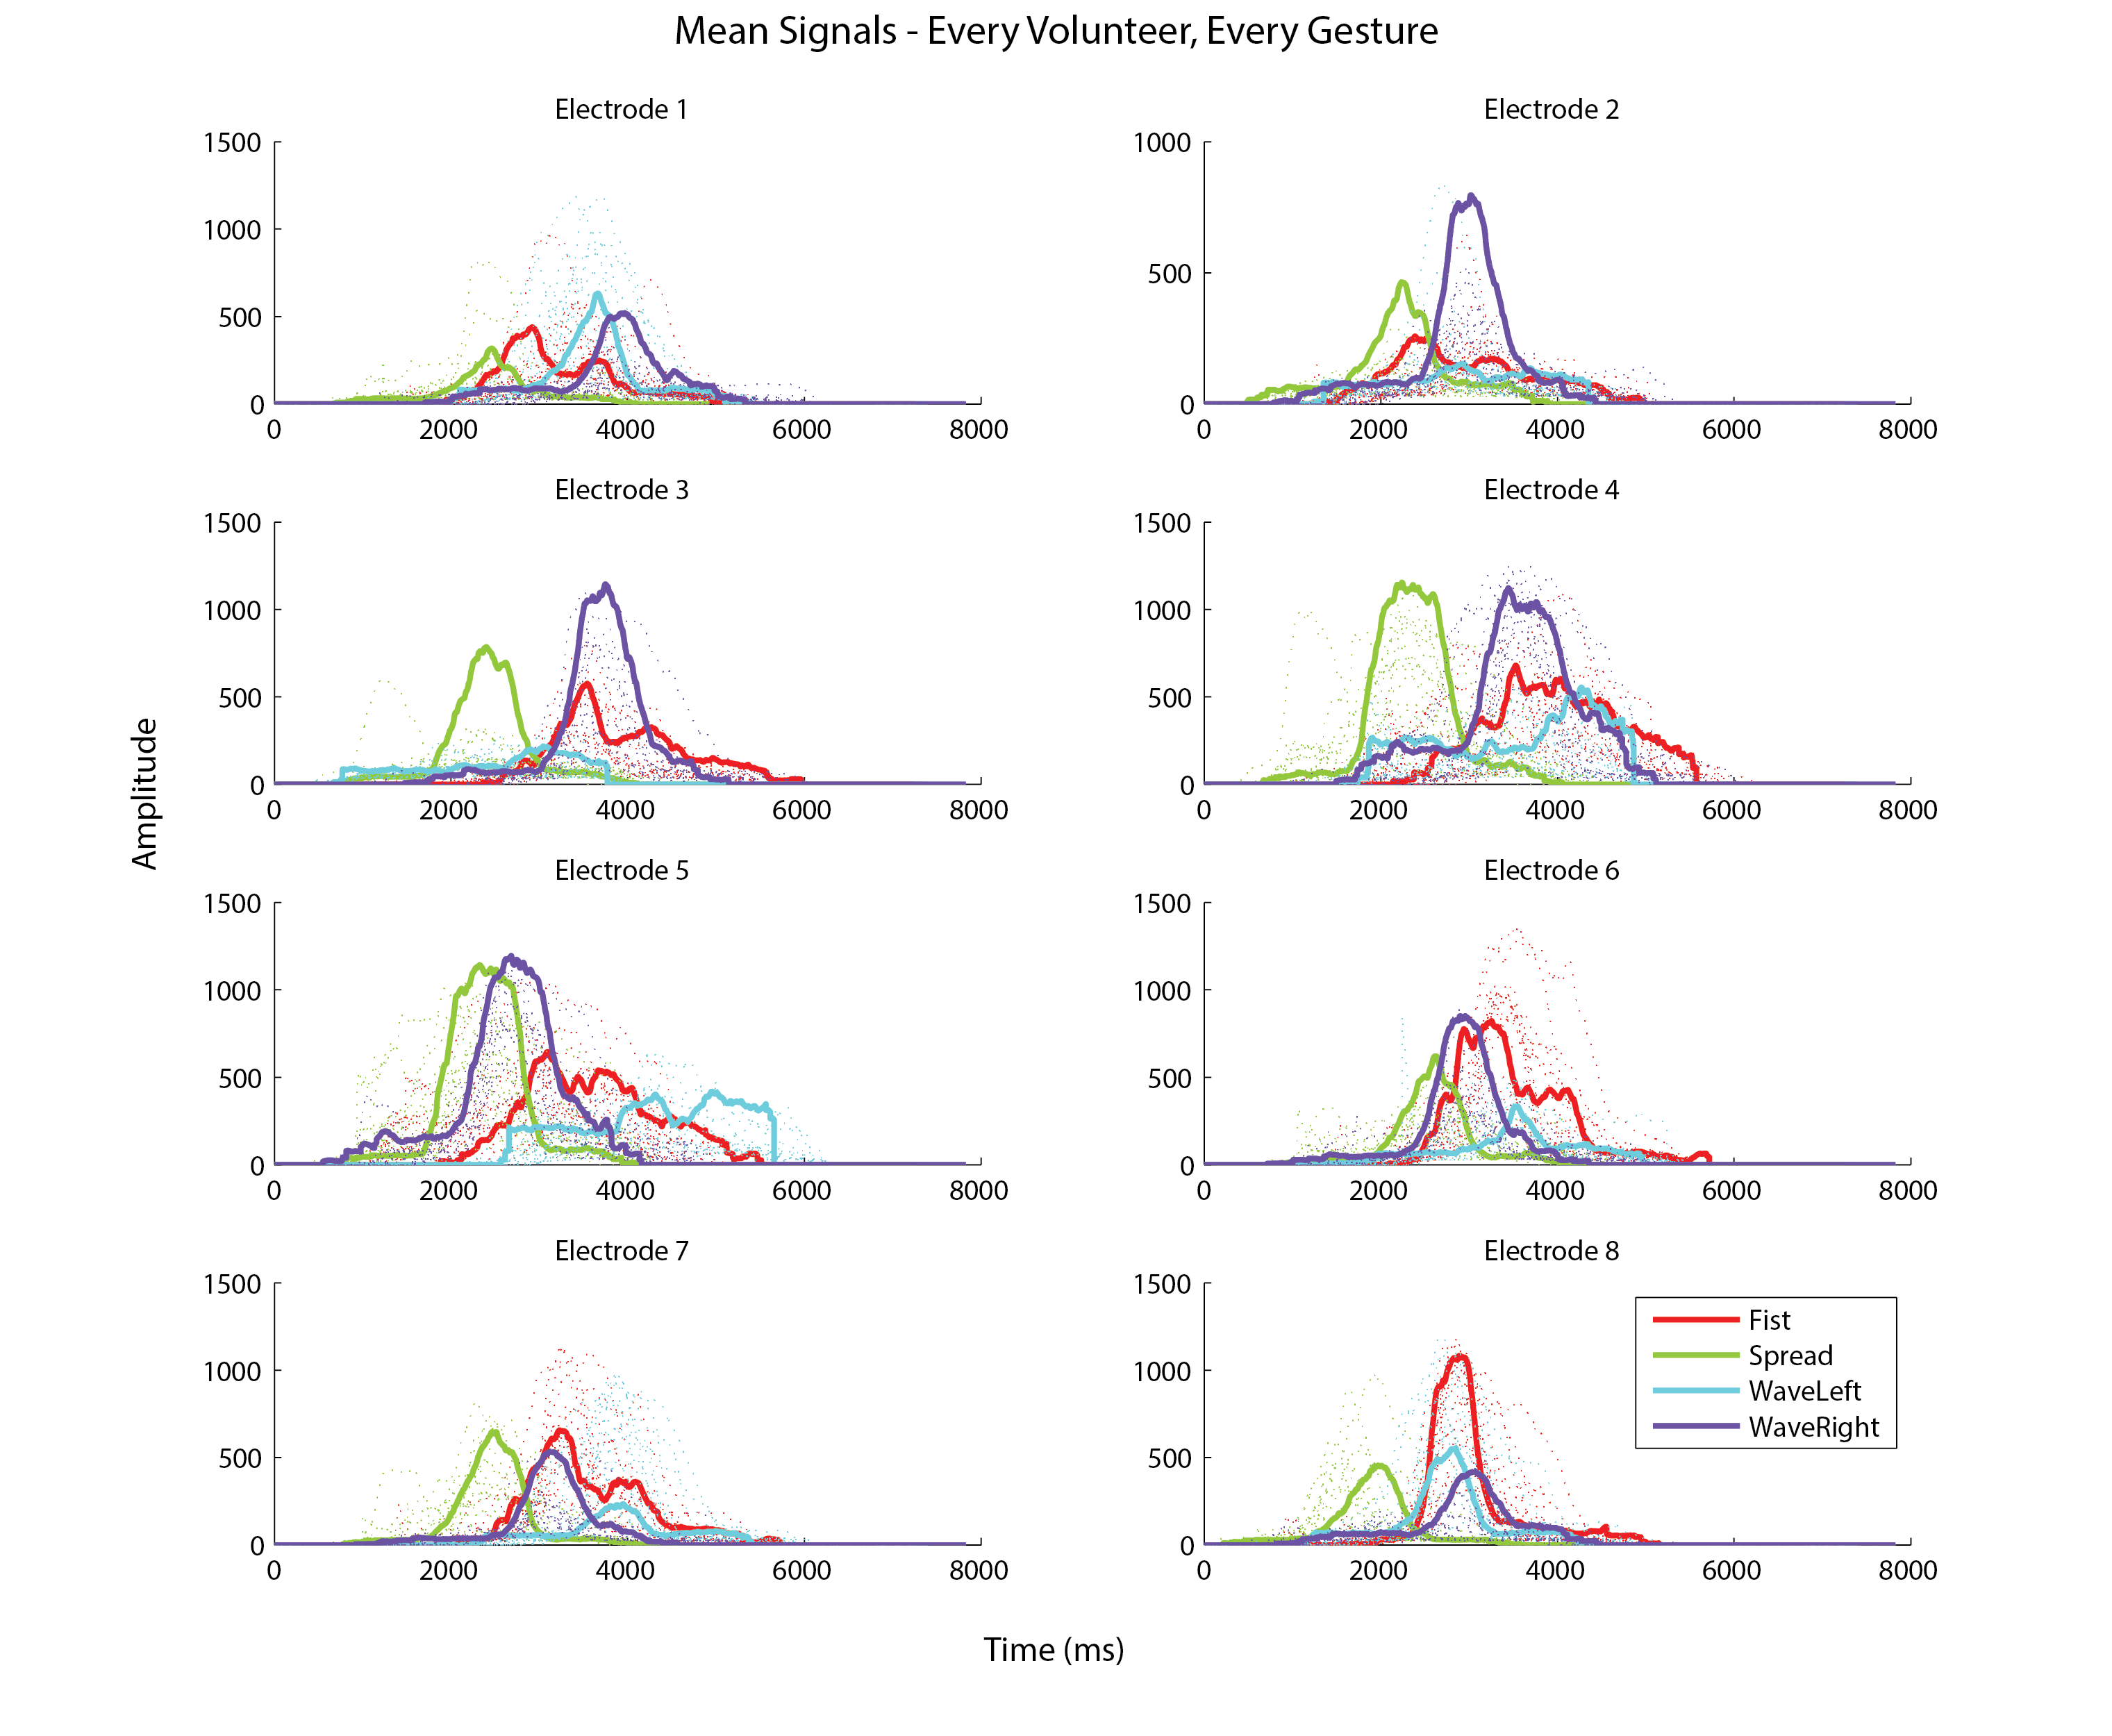
\includegraphics[width=1\columnwidth]{EMG/Mean_All}
    \caption{Plots of the mean signals for each volunteer for each gesture.}
    \label{Mean_All}
    \end{figure}

\subsubsection{Future Work} \\
These results could be further investigated by [adding some small changes to the experimental method].
It would be beneficial to measure the raw data from the Myo armband in tandem as the accuracy of the built-in gesture recognition algorithm is being tested for each volunteer. By doing this, a raw data sample could be recorded and associated with an accuracy value, allowing us to further investigate the relationship between signal shape, length, and amplitude and the algorithm's accuracy when interpreting these signals. 

It would also be worthwhile to compare the accuracy of the built-in gesture recognition algorithm to similar existing algorithms published in scientific literature.

Finally, these tested and refined algorithms could be applied in order to control robotic devices, such as prosthetic limbs and robotics arms, which are already being controlled using similar algorithms and medical-grade EMGs.

\newpage
\FloatBarrier


    \begin{figure}[H]
    \centering
    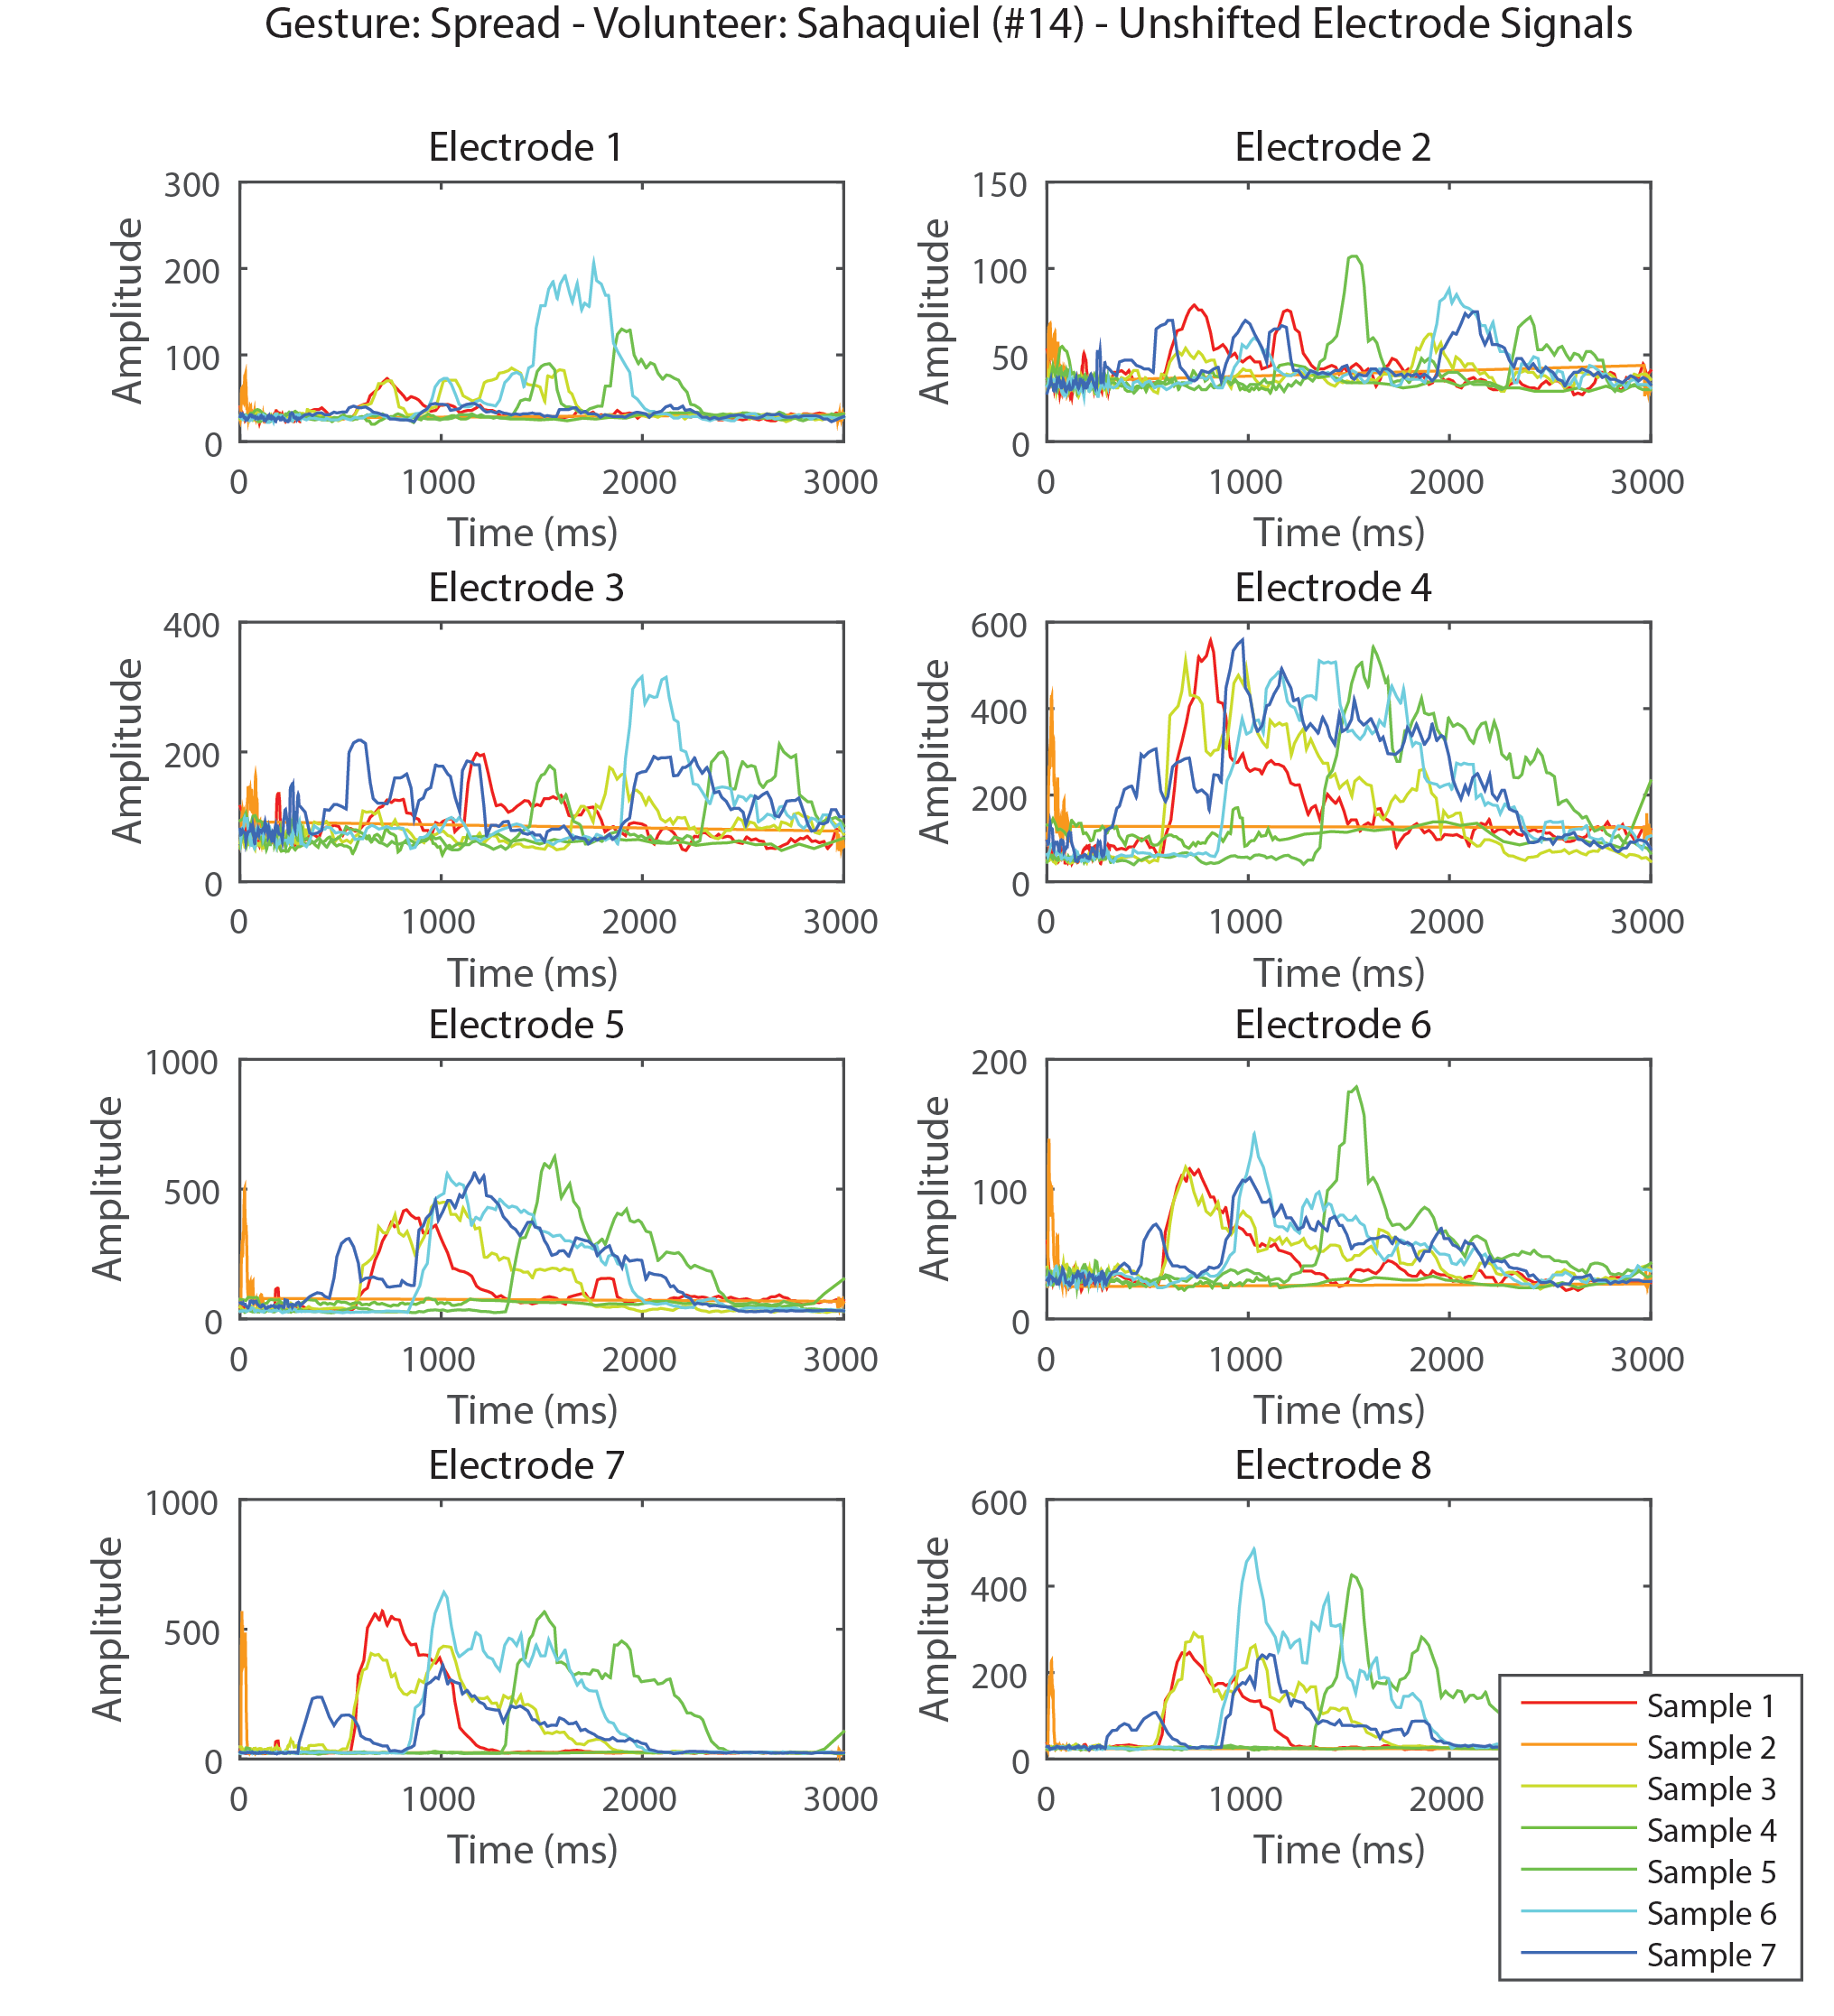
\includegraphics[width=1\columnwidth]{EMG/Spread_Min_Sahaquiel_Unshifted}
    \caption{The raw, unshifted samples generated by volunteer \#14 "Sahaquiel" for the gesture "spread", for each electrode.}
    \label{Spread_Min_Sahaquiel_Unshifted}
    \end{figure}
    
    \begin{figure}[H]
    \centering
    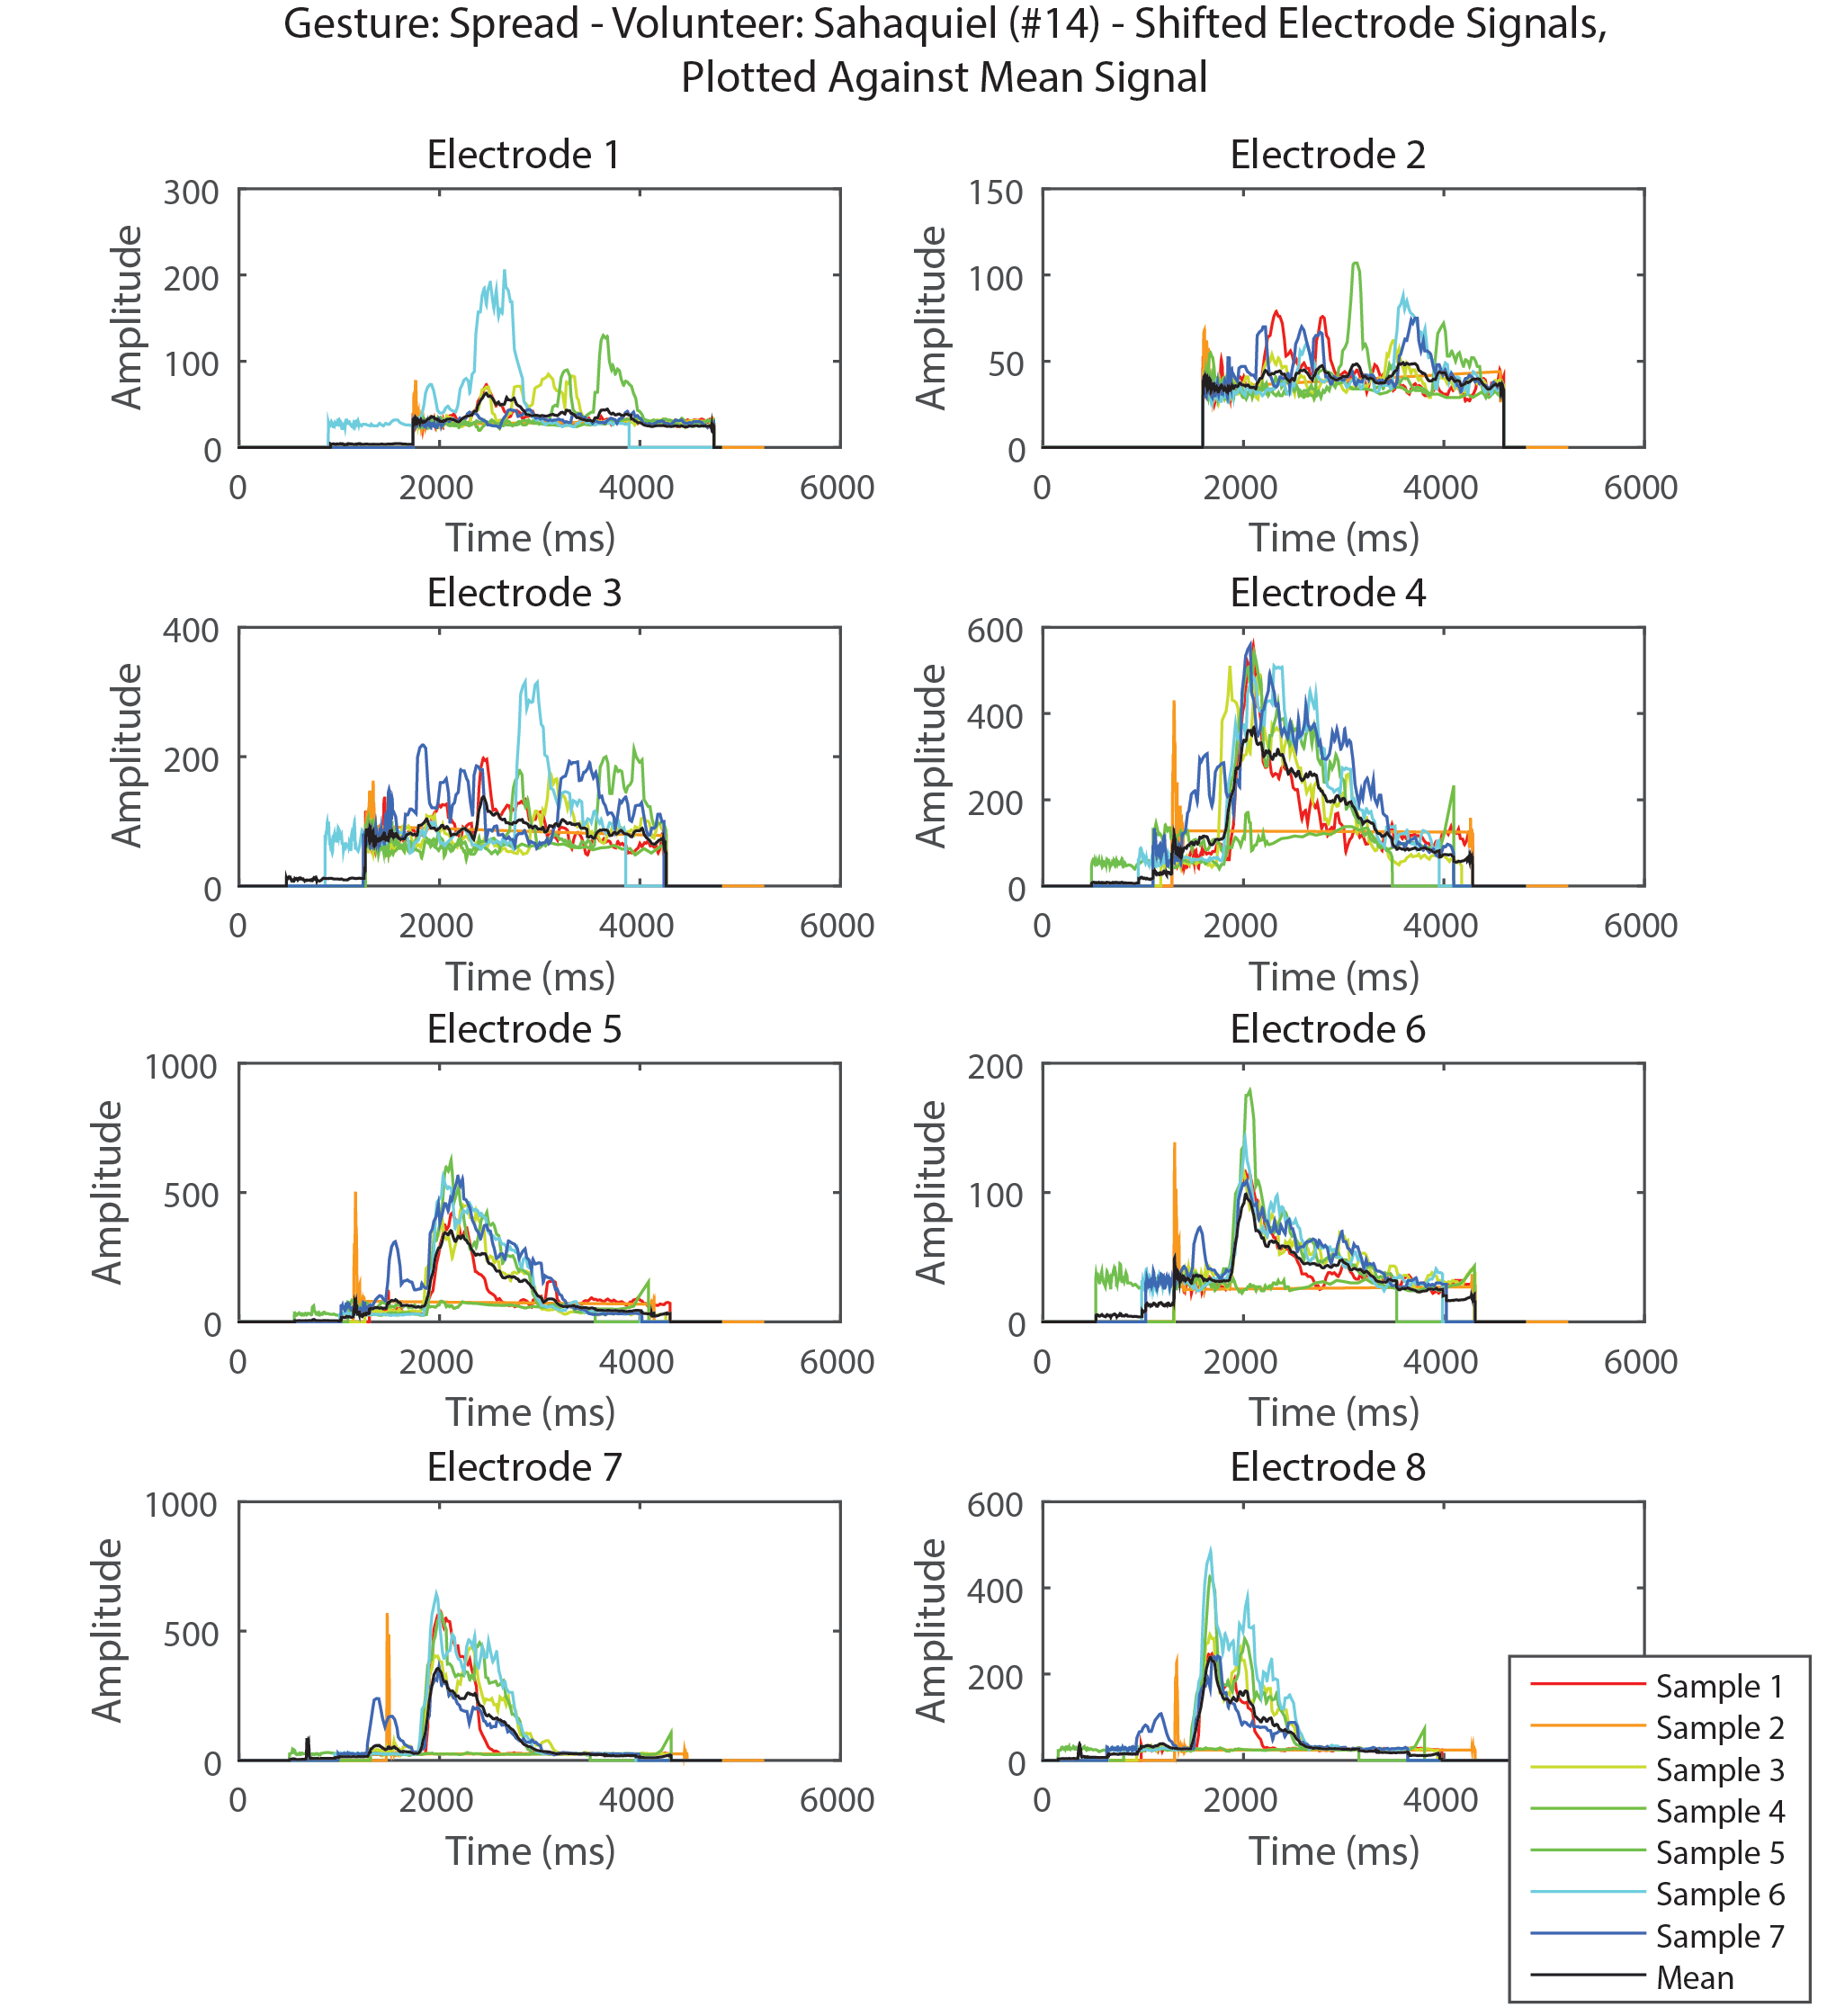
\includegraphics[width=1\columnwidth]{EMG/Spread_Min_Sahaquiel_Shifted}
    \caption{The shifted samples generated by volunteer \#14 "Sahaquiel" for the gesture "spread", for each electrode.}
    \label{Spread_Min_Sahaquiel_Shifted}
    \end{figure}
    
    \begin{figure}[H]
    \centering
    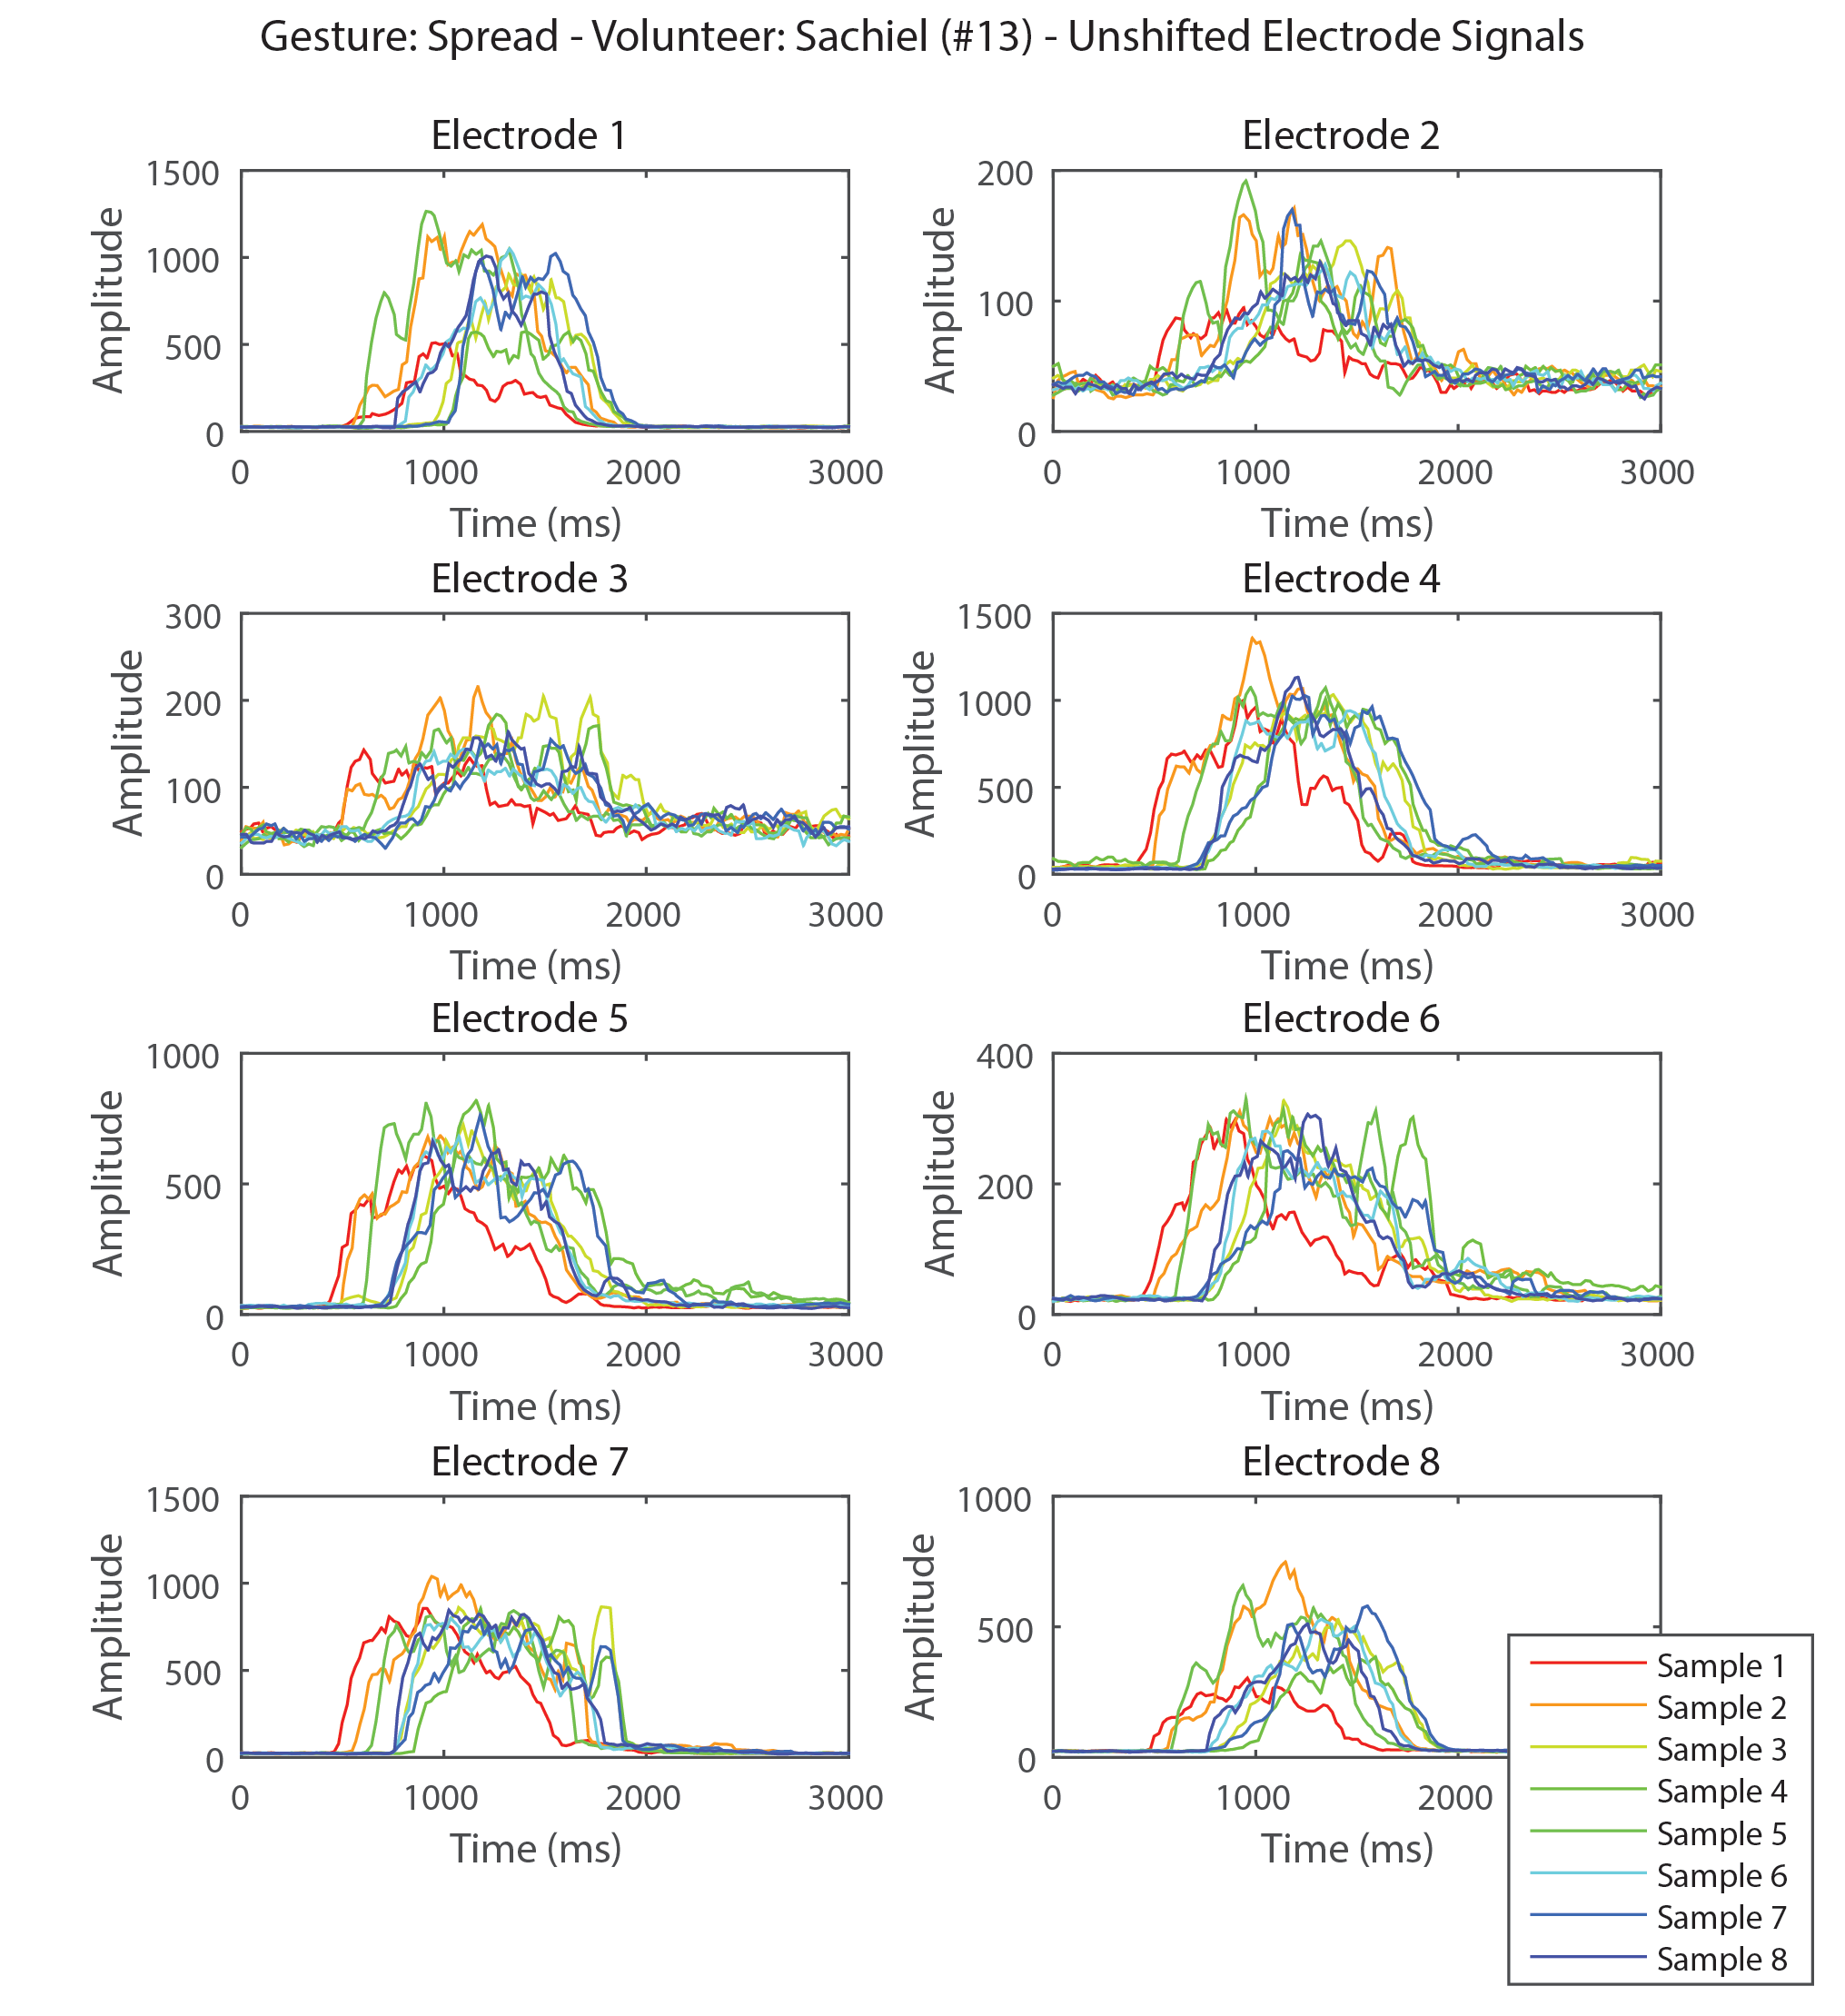
\includegraphics[width=1\columnwidth]{EMG/Spread_Max_Sachiel_Unshifted}
    \caption{The raw, unshifted samples generated by volunteer \#13 "Sachiel" for the gesture "spread", for each electrode.}
    \label{Spread_Max_Sachiel_Unshifted}
    \end{figure}
    
    \begin{figure}[H]
    \centering
    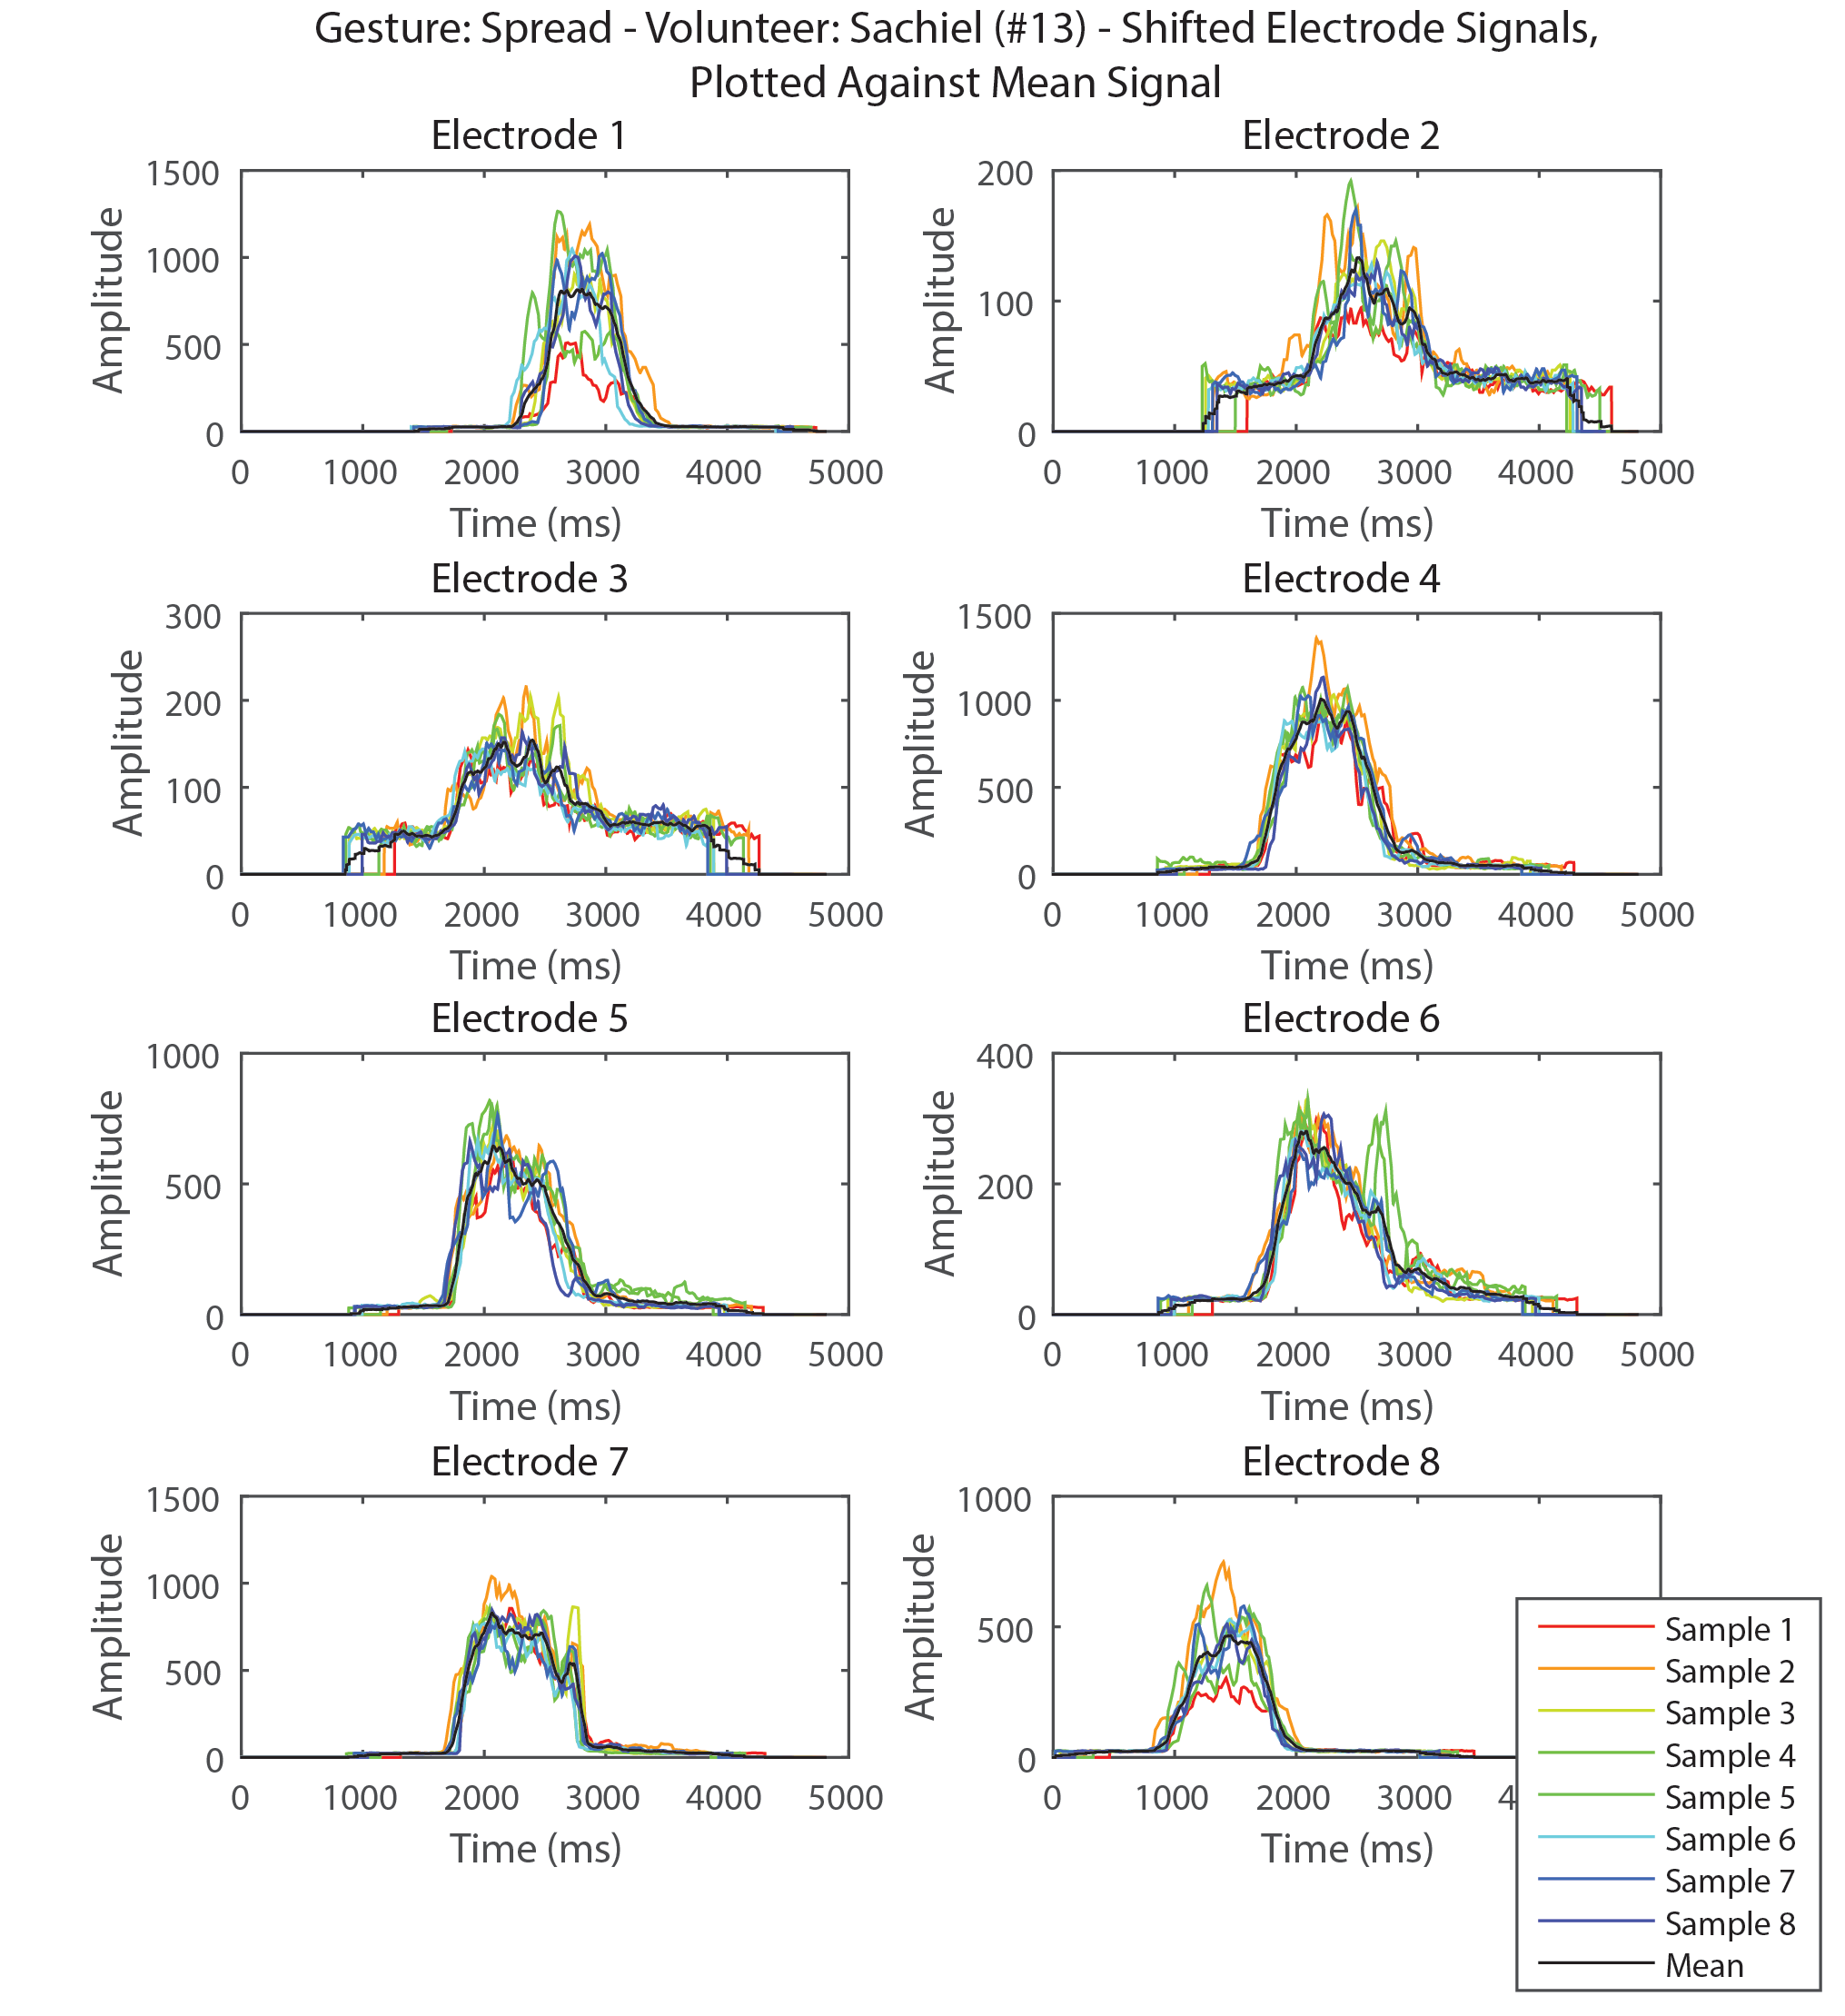
\includegraphics[width=1\columnwidth]{EMG/Spread_Max_Sachiel_Shifted}
    \caption{The shifted samples generated by volunteer \#13 "Sachiel" for the gesture "spread", for each electrode.}
    \label{Spread_Max_Sachiel_Shifted}
    \end{figure}
    \newpage
    
\begin{thebibliography}{1}

\bibitem{IEEEhowto:kopka}
H.~Kopka and P.~W. Daly, \emph{A Guide to \LaTeX}, 3rd~ed.\hskip 1em plus
  0.5em minus 0.4em\relax Harlow, England: Addison-Wesley, 1999.

\end{thebibliography}

\end{document}
